
\section{Wörterbuchproblem}
Menge S mit n Schlüssln aus einem Universum U.
Operationen: INSERT (darauf achten, dass die Balance nicht verloren geht), DELETE, LOOKUP (Im Baum runterlaufen, bis das Element gefunden wurde)
\paragraph{Situationen}
\begin{enumerate}
    \item U linear geordnet, also existiert ein $ \leq $-Test $ \Rightarrow $ Suchbäume
    \item U ist ein Intervall $ \{0,..., N-1\} $ der gesamten Zahlen $ \Rightarrow $ Hashing
\end{enumerate}
\subsection{\underline{zu 1:}}

\paragraph{Randomisierte Suchbäume}
Idee: Benutze Zufallszahlen zur Balancierung eines binären Suchbaums

\paragraph{Binärer Suchbaum (Knoten-Orientiert)}
Schlüssel werden in den n Knoten eines binären Baums gespeichert, sodass im linken Unterbaum des Knotens mit Schlüssel x alle Schlüssel $ < x $ \textbf{und} im rechten Unterbaum alle $ > x $. Balanciert $ \Rightarrow Höhe(T)\leq logn$.  Degeneriert $ \Rightarrow Höhe(T) = O(n)$

\subsection{Definition: Randomized Search Tree (RST)}
Sei $ S=\{x_1,...,x_n\} $ eine Menge von n Schlüsseln. Jedem $ x_i $ wird eine zusätzlich eine Zufallszahl (auch Priorität genannt) $ prio(x_i) $ zugeordnet. $ prio(x_i) $ sind gleichverteilte reelle Zufallszahlen $ \in [0,1] $ (Implementierung wären int-Zahlen, zB 32-bit). \\
Ein RST für S ist eine binärer Suchbaum für die Paare $ (x_i, prio(x_i), 1 \leq i \leq n $, sodass
\begin{enumerate}
    \item normaler Knoten-orientierter Suchbaum für die Schlüssel $ x_i,...,x_n $
    \item Maximumsheap bzgl der Prioritäten. dh $ prio(v) \geq prio(u) $, falls v Parent. ((u,v) sind Knoten in einem Baum). $ \Rightarrow $ Wurzel enthält maximale Priorität.
\end{enumerate}
\textbf{Existenz} durch Algorithmus zum Aufbau (rekursiv).
\begin{itemize}
    \item Wurzel einthält $ (x_i, p_i) $ mit $ p_i = prio(x_i) $ maximal
    \item Linker Unterbaum: RST für $ \{(x_i, p_i)| x_j < x_i \} $
    \item Rechter Unterbaum: RST für $ \{(x_k, p_k)| x_k > x_i \} $
\end{itemize}
Beispiel: $ S=\{1,...,10\} $
\begin{itemize}
    \item Schreibe Tabelle mit Prioriäten und Werten.
    \item Teile die Tabelle beim Maximum und schreibe es in die Wurzel. Wiederhole, bis alle Elemente geschrieben.
\end{itemize}
$ \Rightarrow $ Wenn sich die Prioritäten genauso oder umgekehrt, wie die Schlüssel verhalten, erhält man einen degenrierten Baum. (bzgl $ \leq $). zB $ prio(x_i) = x_i $. Dieser Fall ist sehr unwahrscheinlich, wenn sich bei der Priorität um gleichverteilte Zufallszahlen handelt. 

\subsection{Operationen}

\begin{itemize}
    \item Lookup(x): normale suche in binärem Baum. Kosten $ O(Höhe(T)) $
    \item Insert(x): Füge einen neuen Knoten v als Blatt $ (x, prio(x)) $ gemäß des Schlüssels in den binären Baum ein, wobei $ prio(x) $ neue Zufallszahl (kann die Prio-Ordnung zerstören). Dann: Rotiere v nach oben, bis die Heap-Eigenschaft gilt, also $ prio(v) \leq prio(parent(v)) $. Kosten: O(\#Rotationen) = O(Höhe(T)). Alternativ: normales einfügen in binären Baum in absteigender Reihenfolge der Prioritäten.
    \item DELETE(x): Sei v der knoten mit Schlüssel x (v = Lookup(x)). Kosten: O(\#Rotationen) = O(1 + |L| + |R|)
    \begin{enumerate}
        \item Rotiere v nach unten, bis v ein Blatt ist. R = linkes Rückgrat des rechten Unterbaums von v. L = rechtes Rückgrat des linken Unterbaums. 
        \item Entferne das Blatt.
    \end{enumerate}
    \item Split(y) $ \rightarrow $ $ S_1=\{x\in S | x \leq y\}, S_2=\{x\in S | x \geq y\} $ (Teile den Baum, indem y mit maximaler Priorität zur Wurzel rotiert wird)
    \begin{enumerate}
        \item Insert($ y + \epsilon $) mit Priorität $ \infty $
        \item Entferne die Wurzel 
    \end{enumerate}
    \item Join$ (T_1, T_2 )$: $ S\leftarrow S_1 \cup S_2 $. $T_1$ RST für $S_1$ und $T_2$ RST für $S_2$
    \begin{enumerate}
        \item Konstruiere T (Füge y zwischen Max($S_1$) und Min($S_2$) ein. Voraussetzung: Max($S_1$) < Min($S_2$)
        \item Lösche die Wurzel (Durch runterrotieren des eingefügten Knotens y)
    \end{enumerate}
\end{itemize}

\subsection{Analyse des RST}
Wir analysieren die erwarteten Kosten einer Delete-Operation (Insert $ \rightarrow $ umgekehrtes Delete). Seit T ein RST für die Menge $ \{x_1,...,x_n\}mit x_1 < x_2 < ... < x_n $ der durch Inserts aufgebaut wurde. Bertrachte die Operation Delete($ x_k $) für eine $ k, 1\leq k\leq n $. Für einen Knoten $ x_k $ im Baum T mit Suchpfad $ P_k $, $ L_k $ rechtes Rückgrad von $ T_l $ und $ R_k $ linkes Rückgrad von $ T_r $.  Kosten $ O(|P_k| + |L_k| + |R_k|) $. Wir schätzen die Erwartungswerte 

\subsection{Lemma 1:}
\begin{itemize}
    \item a) E$ (|P_k|) $ = $ H_k + H_{n-k+1} - 1$ $$k-te\ Harmonische Zahl=H_k = \sum_{i_1}^{k}\frac{1}{i}\ H_k \leq ln(x)+1$$
    \item b) E$ (|L_k|) $ = $ 1-\frac{1}{k} $
    \item c) E$ (|R_k|) $ = $ 1-\frac{1}{n-k+1} $
\end{itemize}
\paragraph{Beweis} Betrachte eine Permutation $ \pi:[1..n] \rightarrow [1..n] $ (bijektive Abbildung), die die Schlüssel absteigend nach ihren Prio Werten sortiert. Dann gilt: 
\begin{enumerate}
    \item Jede Permutation $ \pi $ ist gleichwahrscheinlich (Wahrscheinlichkeit $ \frac{1}{n!} $), da die Prioritäten gleichverteilte Zufallszahlen sind.
    \item Man erhält den selben binären Baum durh einfügen der Schlüssel in einen unbalancierten Baum in der Reihenfolge, die $ \pi $ angibt. $ \rightarrow $ gleiches Vehalten, wie ein zufälliger binärer Baum.
    \item Baum wächst nur an den Blättern.
\end{enumerate}
Trick: arbeite ab jetzt mit zufälliger Permutation statt den Prioritäten. $ \rightarrow $ normaler Binärbaum mit zufälliger Einfügereihenfolge.
\paragraph{Teil a) des Lemmas} $P_k $ ist Suchpfad für Knoten $x_k $. Seien $ P'_k $ und $ P''_k $ Teilfolgen von $ P_k $ mit: $ \forall v \in P'_k, key(v)\leq x_k $ und $ \forall u \in P''_k, key(u)\geq x_k $. 
\begin{proof}
Beobachtungen:
\begin{enumerate}
    \item $ |P_k| = |P'_k| + |P''_k| - 1 $ ($ x_k $ in beiden Teilfolgen)
    \item $ P'_k = $ Menge der knoten v mit:
    \begin{itemize}
        \item Wenn v eingefügt wird, gilt key(v) ist maximal mit key(v)$ \leq x_k $
    \end{itemize}
    \item $ P''_k = $ Menge der knoten u mit:
    \begin{itemize}
        \item Wenn u eingefügt wird, gilt key(u) ist minimal mit key(u)$ \geq x_k $
    \end{itemize}
\end{enumerate}
Wir zeigen
\begin{enumerate}
    \item E($ |P'_k| $) = $ H_k $
    \item E($ |P''_k| $) = $ H_{n-k+1} $
\end{enumerate}
\underline{zu 1)} K mögliche Kandidaten für $ P'_k \{x_1,...,x_k\}$. Spiel: Ziehe zufällig Schlüssel aus $\{x_1,...,x_k\}$. E($ |P'_k| $) = Erwartungswert, wie of ein Kandidat gezogen wird, der $ \geq $ als alle vorher gezogenen ist (neues Maximum). $ A^k = E(|P'_k|)$ (Spiel A)

$$A^k = \sum_{i=1}^k \frac{1}{k} \cdot (1 + A^{k-i})$$

Im Zug $ x_i $ schließt $ x_1 ... x_i $ au. Dann gleiches Spiel mit K-i Kandidaten.

$$A^k = \frac{1}{k} (k + \sum^{k}_{i=1} A^{k-i}) $$
$$ = 1 + \frac{1}{k} \sum^{k}_{i=1} A^{k-i}$$ 

Wir zeigen durch Induktion über k, dass $ A^k = H_k $

\paragraph{IA}
$$ = 1 + \frac{1}{k} \sum^{k}_{i=0} H_i$$ 
Eigenschaften der harmonischen Zahlen:
\begin{enumerate}
    \item $$ \sum^{k}_{i=0} H_i = k \cdot (H_k -1 )$$
    \item $$ H_k \leq 1 + lnk$$ 
\end{enumerate}
aus 1) folgt: 

$$A^k = 1 + \frac{1}{k} \cdot k \cdot (H_k - 1)$$
$$    = 1 + H_k - 1$$
$$    = H_k$$
Der Erwartungswert ist ist gleich der k-ten Harmonischen Zahl. $E(P'_k) = H_k$. Abschätzung von $E(P''_k) =: B^k$. (Spiel B) kandidaten $ \{ x_k ... x_n\} $: Zähle, wie of ein neues Minimum gezogen wird. Dann sieht man leicht, dass 
$$B^k = H_{n-k+1}$$
Beweis: symmetrisch.
$$E(|P_k|) = E(|P'_k|) + E(|P''_k|) - 1 $$
$$ = A^k + B^k - 1 $$
$$ = H_k + H_{n-k+1} - 1 $$

\end{proof}

\paragraph{Teil b) des Lemmas}

\begin{proof}{$L_k$ und $R_k$}
Seien $ L_k = v_1, ... , v_l $ und $ R_k = u_1, ... , u_m $
\paragraph{Erwartungswerte}
Spiel C: Ziehe zufällig Elemente aus $ \{x_1 ... x_n \} $.
Sobald $ x_k $ gezogen wird: ??? Trigger ???
Sei $ C^k $ der Erwartungswert dieses Spiels, dh $ C^k = E(|L_k|) $.

$$ C^k = \frac{1}{k} \cdot A^{k-1} + \sum_{i=1}^{k-1} \frac{1}{k} \cdot C^{k-i}$$
im 1. Zug $ x_k $, dass Spiel mit k-1 Kandidaten (alle kleiner, als $ x_k $).

$$ C^k = \frac{1}{k} (\cdot H_{k-1} + \sum_{i=0}^{k-1} \cdot C^{i})$$

Trick: Schätze die Differenz zweier aufeinanderfolgender $ C^i $s = $ \delta_j = C^{j+1} - C ^j $ ab.

$$\Rightarrow C^k = \sum_{j=1}^k \delta_j + C^0$$

Beatrachte: 
$$ (j + 1) \cdot C^{j+1} - j \cdot C ^j $$
$$ = (j + 1) \frac{1}{j+1} (H_j + \sum_{i=0}^j C^i) - j \frac{1}{j} (H_{j-1} + \sum_{i=0}^j C^i)$$
$$ = H_j + \sum_{i=0}^j C^i - (H_{j-1} + \sum_{i=0}^j C^i)$$
$$ = H_j - H_{j-1} + C^i$$ 
$$ = \frac{1}{j} + C^j$$
Wir wissen nun, dass
$$ (j + 1) \cdot C^{j+1} - j \cdot C ^j  = \frac{1}{j} + C^j$$
$$ \frac{1}{j} = (j+1) C^{j+1} - (j+1) \cdot C^j $$
$$ \frac{1}{j(j+1)} = C^{j+1} - C^j = \delta_j $$
$$ \Rightarrow \delta_j = \frac{1}{j(j+1)} = \frac{1}{j} - \frac{1}{j+1}$$
$$ C^k = \sum_{j=1}^{k-1} \delta_j = \sum_{j=1}^{k-1} (\frac{1}{j} - \frac{1}{j+1})$$
$$ = 1 - \frac{1}{k}$$

\end{proof}


\paragraph{Teil c) des Lemmas}
Spiel $ D^k = E (|R_k|) $: Wie oft wird ein neues Minimum größer $ x_k $ gezogen, nachdem $ x_k $ gezogen wurde (Trigger).

\begin{proof}
symmetrisch:

$$ D^k = \frac{1}{n-k+1} \cdot B^{k-1} + \sum_{i=1}^{k-1 ??} \frac{1}{n+k-1} D^{i-k ??} $$
\textbf{...}
$$ D^k = 1 - \frac{1}{n-k+1}$$

\end{proof} 

\paragraph{Satz} Sie T ein RST für eine Menge von n Schlüsseln. Dann gilt:
\begin{enumerate}
    \item Die erwartete Laufzeit fpr Insert, Delete und Lookup ist O(logn)
    \item Die erwartete Zahl der Rotationen bei Delete ist < 2
\end{enumerate}
\paragraph{Beweis}
\begin{enumerate}
    \item Kosten von Lookup = $ O(|P_k|) $, Insert und Delete = $ O(|P_k| + |L_k| + |R_k|) $
    Kosten: $ O(H_k + H_{n-k+1} + 1 - \frac{1}{k} + 1- \frac{1}{n-k+1}) = O(H_n) = O(lnn) = O(logn)$
    \item Erwartete Zahl der Rotationen: $ E(|L_k|) + E(|R_k|) < 2 $
\end{enumerate}


\section{Hashing}

\subsection{Hashing mit offener Adressierung}
Tafel T $ [0, ..., m-1], m \leq n, |S| = n $
Verwende die Folge von Hashfunktionen $ h_0, h_1 $ 
$$ h_i(x) = f(x) + i \cdot g(x), i = 0,1,...$$
Häufig verwendet wird
$$ h_i(x) = (x \cdot mod m + i)\cdot mod m $$
$\rightarrow$ Linear Probing.\\
Idee
\begin{figure}[h]
    \begin{center}
        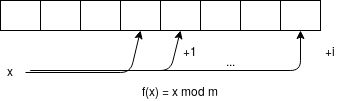
\includegraphics[width=10cm]{offeneadressierung.png}
        \caption{Idee: Offene Adressierungs-Tabelle}
        \label{fig:}
    \end{center}
\end{figure}

\paragraph{Operationen} Tafelposition T[i] belegt oder frei.
\begin{itemize}
    \item Init: alle frei
    \item Insert(x): betrachte die Tafelpositionen $T[h_0(x)], T[h_1(x)], T[h_2(x)]$ bis $ T[h_i(x)] $ frei und speicher x dort ab.
    $ T[h_i(x)] \leftarrow x $ und markiere $ T[h_i(x)]$ als belegt. Voraussetzungen:
    \begin{enumerate}
        \item $ m \leq |S| = n $
        \item $ h_i(x) $ frei $ i = 0,1,2,... $ muss alle Tafelpoitionen durchlaufen
    \end{enumerate}
    \item Lookup(x): Teste die Tafelpoition $ T[h_i(x)] $ für $ i=0,1,2,... $ bis entweder $ T[h_i(x)] = x $ erfolgreich oder $ T[h_i(x)] $ ist frei. \textbf{Terminiert nicht}, wenn m=n und die Tafel voll ist und das gesuchte Element nicht vorhanden ist. Daher idR $ m \geq n $
    \item Delete(x): (Idee 1):
    \begin{enumerate}
        \item $ j \leftarrow Lookup(x) $ 
        \item $ T[j] \leftarrow frei $, dann sind auf j folgende Elemente nicht mehr erreichbar.
    \end{enumerate}
    (Idee 2):
    \begin{enumerate}
        \item Dritter Zustand: 'gelöscht' (Details: Übung)
    \end{enumerate}
\end{itemize}



\subsection{Perfektes Hashing}
\textbf{Situation:} Statische Menge  S von n Schlüsseln aus $ [0,..,N-1] $. \textbf{Ziel:} Speichere S in einer Tafel der Größe O(n), sodass Lookup in Zeit O(1) realisiert werden kann (N >> n, N sehr viel größer, als n). \textbf{Andere Formulierung:} Finde einer Hashfunktion $ h: [0,..., N-1] \rightarrow [0,...,S-1] $ mit 
\begin{enumerate}
    \item S = Größe der Tafel und S = O(n)
    \item h injektiv auf S
\end{enumerate}
Zur Konstruktion oder Auswahl einer solchen Funktion Hashfunktion verwenden wir ein probabilitisches Verfahren (Zufallsverfahren).
\paragraph{Idee} 2-stufiges Hashing-Schema (Hashing-Verfahren)
\begin{figure}[h]
    \begin{center}
        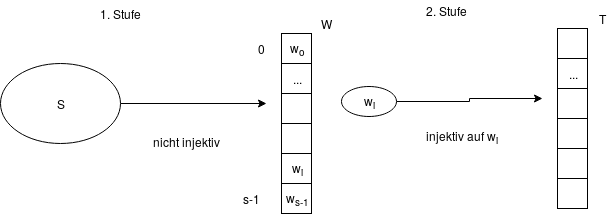
\includegraphics[width=10cm]{perfekthashing.png}
        \caption{Idee: Perfekt Hashing Tabellen}
        \label{fig:}
    \end{center}
\end{figure}

Sei p eine Primzahl mit p > N und $ S \in \mathbb{N} $ (Tafelgröße). Betrachte folgende Hashfunktionen:

$$ h_k:[0,...,N-1] \rightarrow [0,...,S-1] $$ mit $ h_k(x)= ((k \cdot x) mod p) mod s  $ für alle $ 1 \leq k \leq p-1 $ (Modulo Primzahl ergibt einen Restkörper, zB Inverses der Multiplikation). Diese Funktionen sind im Allgemeinen nicht injekt, dh $ h_k $ verteilt die Menge S auf s Buckets $ W_0^k, W_1^k, W_{s-1}^k $. 
$$ \Rightarrow W_i^k  = \{x\in S | h_k(x) = i\} $$

$ h_k $ injektiv auf $ S \Leftrightarrow |W_i^k| \leq 1 $ für $ 0 \leq i \leq s-1 $

\paragraph{Lemma 1: } Für jede Menge $ S \subseteq \{0,..., N-1 \}, |S| = n $ gilt $ \exists k, 1 \leq k \leq p-1 mit $

$$ \sum_{i=0}^{s-1} \binom{|W_i^k|}{2} < \frac{n^2}{s}$$
(Anzahl der Kollisionen < $\frac{n^2}{s}$). \\

\paragraph{Beweis} zunächst: Behauptung.
$$ \sum_{k=0}^{p-1} \sum_{i=0}^{s-1} \binom{|W_i^k|}{2} <  (p-1)\frac{n^2}{s}$$

Daraus folgt das Lemma (indirekt). Annahme, das Lemma 1 gilt nicht, dh $\forall 1\leq k\leq p-1: $

$$ \sum_{i=0}^{s-1} \binom{|W_i^k|}{2} \geq \frac{n^2}{s}$$

$$ \Rightarrow  \sum_{i=0}^{s-1} \binom{|W_i^k|}{2} \geq \frac{n^2}{s}$$
Widerspruch zur Behauptung!

\begin{proof}[Beweis zur Behauptung]

$$ (1)\sum_{k=0}^{p-1} \sum_{i=0}^{s-1} \binom{|W_i^k|}{2}$$
= Anzahl der Paare $ (k, \{x,y\} $, $ x\neq y$ und $ h_k(x) = h_k(y) $ (Anzahl der Kollisionen).\\
Wir schätzen zunächst den Betrag für 2 feste Werte $ x \neq y $ zur Behauptung ab.\\

Sei also $ x \neq y $: \\
(1) = Anzahl aller Ks mit $ (k\cdot x\cdot mod p)mods = (k \cdot y\cdot modp)mods $
\[ \Leftrightarrow ((k\cdot x\cdot mod p)-(k\cdot y\cdot mod p))mods = 0 \]
\[ k\cdot x\cdot mod p - k\cdot y\cdot mod p = i \cdot s \text{ für ein } i\in \mathbb{Z} \]
\[k\cdot (x-y) mod p = i\cdot s \]
Es gibt maximal $ \frac{2(p-1)}{s} $ mögliche Lösungen. Da p eine Primzahl ($ \mathbb{Z}_p $ ist ein Körper) hat jede dieser Gleichungen höchstens 1 Lösung für k.
$ \Rightarrow $ Beitrag eines festen Paares $ x \neq y $ zu (1) ist maximal $ \frac{2(p-1)}{s} $ \\

\[ \Rightarrow (1) \leq \binom{n}{2} \cdot \frac{2(p-1)}{s}\]
\[ = \frac{n(n-1)}{2} \cdot \frac{2(p-1)}{s}\]
\[ < \frac{n^2(p-1)}{s}\]

\end{proof}

\paragraph{Folgerung 1} (aus Lemma 1) \\
Für s=n (dh Tafel der Größe n): 
$$\exists k ,1 \leq k \leq p-1 \text{ mit } \sum_{i=0}^{n-1} |W_i^k|^2 < 3n$$

\begin{proof}[Beweis für Folgerung 1]
Betrachte Lemma 1 für s=n

\begin{flalign}
\exists k: \sum_{i=0}^{n-1}\binom{|W_i^k|}{2} &< n \\
\sum_{i=0}^{n-1} \frac{|W_i^k| \cdot(|W_i^k| - 1)}{2} &< n\\ 
\sum_{i=0}^{n-1} |W_i^k| \cdot(|W_i^k| - 1) &< 2 n \\
\sum_{i=0}^{n-1} |W_i^k|^2  &< 2 n + \sum_{i=0}^{n-1} |W_i^k|(=n) \\
 &<3n
\end{flalign}

\end{proof}


\paragraph{Folgerung 2} Für $ s = n^2 $ dh quadratische Tafelgröße. \\
$ \exists k' : 1\leq k \leq p-1 $, sodass die Hashfunktion
$$ k_{k'}:x \rightarrow (k'x\cdot modp) mods $$
injektiv auf S ist dh $ |W_i^k| \leq 1 \text{ für } 0\leq i \leq s-1 $.\\
$\Rightarrow$ Für Tafeln mit quadratische Größe existiert eine perfekte (injektive) Hashfunktion.

\begin{proof}[Beweis für Folgerung 2]
Betrachte Lemma 1 mit $ s= n^2 $

\begin{flalign}
\exists k': \sum_{i=0}^{n^2-1}\binom{|W_i^k|}{2} &< 1 \\
\Rightarrow  |W_i^k| &\leq 1\\
\Rightarrow  h_{k'}\text{ ist injektiv auf S}
\end{flalign}
(zu 6): dh Keine Kollisionen, bzw Doppeltbelegung in den $ W_i^k $

\end{proof}

Folgerung 2 zeigt Perfektes Hashing mit quadratischem Platz. Vermeidung des quadratischen Platzbedarfs durch ein 2-stufigen Hashing-Schema:

\begin{itemize}
    \item Stufe 1: Wähle ein k gemäß Folgerung 1, dh Tafelgröße s=n und Hashfunktion $ h_k $ mit $ \sum_{i=0}^{n-1} |W_i^k| < 3n $
    \item Stufe 2: Für jedes nicht-leere Bucket $ W_i^k $ der ersten Stufe verwende iene Tafel der Größe $ s_i = |W_i^k|^2 (0 \leq i \leq n-1) $ und wähle ein $k_i$ gemäß Folgerung 2, dh $ h_{k_i} $ ist injektiv auf $ W_i^k $
\end{itemize}

\begin{figure}[h]
    \begin{center}
        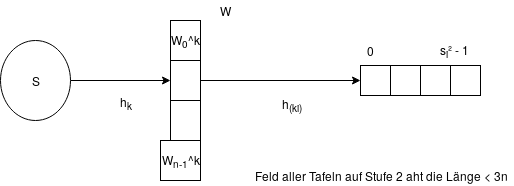
\includegraphics[width=15cm]{2stufenhashing.png}
        \caption{Konzept 2-Stufen Hashing}
        \label{fig:}
    \end{center}
\end{figure}


\subsubsection{Datenstruktur} 4 Felder + Variable k
\begin{itemize}
    \item Variable k: ($ h_k $ der 1. Stufe)
    \item k[0,...,n-1]: k[i] ist $ k_i $ der 2. Stufe
    \item Size[0,...,n-1]: Size[i] = $ |W_i^k| $ Bucketgrößen der 1. Stufe
    \item Ptr[0,...,n-1]: Pointer auf die Hashtafeln der 2. Stufe. Ptr[i] zeigt auf die Tafel B[0,...,Size[i]$^2$-1]
    \item T[0,...,3n]: Gesamtspeicherplatz aller B-Tafeln der 2. Stufe
\end{itemize} 

\begin{figure}[h]
    \begin{center}
        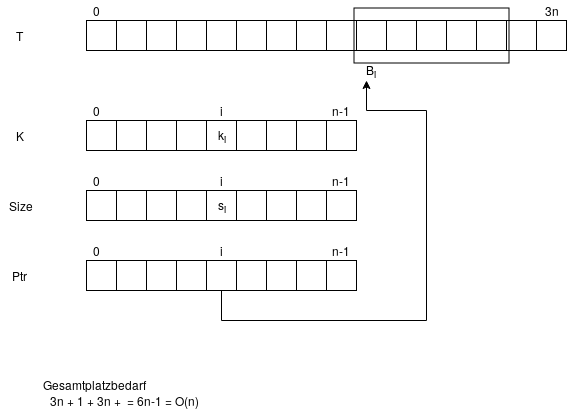
\includegraphics[width=15cm]{datenstruktur.png}
        \caption{Datenstruktur: Perfekt Hashing}
        \label{fig:}
    \end{center}
\end{figure}

\paragraph{Abspeichern eines Elements x}
\begin{flalign}
i &\leftarrow (k \cdot x mod p ) mod n\\
k' &\leftarrow K[i]\\
s' &\leftarrow Size[i]\\
j &\leftarrow (k'\cdot x mod p) mod s'\\
Ptr[i][j] &\leftarrow x
\end{flalign}

\begin{algorithm}
    
\end{algorithm}



\subsubsection{Aufbauzeit der Datenstruktur}
Wir findet man die k bzw k' Werte der ersten und zweiten Stufe (gemäß Folgerung 1 und 2). Aus Folgerungen 1 und 2 folgt: Es existiert immer mindestens ein Wert für k (dh eine geeignete Hashfunktion $ h_k $). \textbf{Aufbaualgorithmus:} Teste alle k-Werte. Auf 1. und 2. Stufe\\
\begin{algorithm}[H]
\SetKwProg{Def}{def}{:}{end}
\Def{Aufbau}{
    \For{$k=1$ \KwTo $p-1$} {
        1.Stufe: Teste ob $ \sum_{i=0}^{n-1} |W_i^k|^2 < 3n $\;
    }
}
\end{algorithm}
Kostet im worst case $ O(p \cdot n) = O(n \cdot N) $\\

2.Stufe für jedes Bucket $ W_i^k $ \\
\begin{algorithm}[H]
\SetKwProg{Def}{def}{:}{end}
\Def{Aufbau}{
    \For{$k'=1$ \KwTo $n$} {
        Teste ob $ h_{k'} \text{ injektiv auf } W_i^k$\;
    }
}
\end{algorithm}
Kostet für $ W_i^k O(p \cdot |W_i^k|$ für alle Buckets $ W_i^k (0 \leq i \leq n)$. Gesamtlaufzeit:

\begin{flalign}
O(\sum_{i=0}^{n-1} p\cdot|W_i^k|)    
\end{flalign}


Eine genauere Analyse zeigt, dass es viele  k-Werte mit den geforderten Eigenschaften gibt.

\paragraph{Folgerung 3} (aus Lemma 1) \\
Für mindestens die Hälfte aller k, $ 0 \leq k \leq p-1 $, gilt 
$$ \sum_{i=0}^{n-1}|W_i^k|^2 < 5n (s=n)$$

\paragraph{Folgerung 4} (aus Lemma 1) \\
Für mindestens die Hälfte aller k', $ 0 \leq k' \leq p-1 $, gilt 
$$ h_{k'}:x\rightarrow (k'\cdot x\ mod p) mod 2 \cdot  n^2 $$
ist injektiv auf S (angedwandt: $ W_i^ks $. Beweis analog zum Beweis der Folgerung 1 und 2.

\paragraph{Änderungen in der Datenstruktur} Auf 2.Stufe Tafelgrößen verdoppeln, dh jeweils Größe $ 2 \cdot |W_i^k|^2 $. Platzbedarf der 2.Stufe:

$$ \sum_{i=0}^{n-1} 2- |W_i^k|^2 = 2 \sum_{i=0}^{n-1} |W_i^k|^2 < 10n $$

Insgesamt: Platz 13n = O(n). 
\subparagraph{Aufbau}
\textbf{Stufe 1:} Wähle ein zufälliges $ k \in \{1,...,p-1 \} $ bis Folgerung 3 erfüllt. Wahrscheinlichkeit daür ist jeweils $ \geq \frac{1}{2} $. \textbf{Frage:} Wie hoch ist der Erwartungswert für die Anzahl der Tests. Analog zum Münzwurf: Wie viele Würfe, bis eine bestimmte Seite erscheint?
Erwartungswert für diese Zahl (Integrierende Reihe): 
$$ \sum_{i=0}^\infty \frac{1}{2^i} \cdot i = \frac{0.5}{(1-0.5)^2} = 2 $$
Erwartete Laufzeit für Stufe 1 ist dann $ O(2 \cdot |S|) = O(n) $. Analog für Stufe 2: Erwartete Zahl der Tests = 2. $ \Rightarrow $ Gesamtlaufzeit O(n).

\subsubsection{Zusammenfassung}
Man kann eine Menge S von n Schlüsseln aus $ [0,...,N-1] $ so abspeichern, dass gilt 
\begin{enumerate}
    \item Platubedarf ist O(n)
    \item Erwartete Aufbauzeit O(n)
    \item Zugriffszeit (Lookup) O(1) worst-case
\end{enumerate}

Dynamisierung ist möglich (Dynmaic Perfect Hashing). Idee: Zeigen, dass die gewählten k-Werte mit großer Wahrscheinlichkeit für weitere Schlüssel funktionieren.


\section{Planare Graphen}
Literatur: Nishizekim und Chiba (Planar Graphs). Graph kann in die Ebene gezeichnet werden, ohne dass sich Kanten kreuzen. Wir betrachten ungerichtete Graphen G=(V,E).
\subsection{Definition}
\begin{enumerate}
    \item Ein Graph G=(V,E) ist planar, wenn G eine planare Zeichnung hat.
    \item Eine planare Zeichnung von G ordnet jedem Knoten v einen Punkt $ p \in \mathbb{R}^2 $ (Ebene) zu, $ p = pos(x) $ heißt die Position von v, und jeder Kante $ (v,w) $ eine stetige Kurve im $ \mathbb{R}^2 $ mit den Endpunkten $ pos(v) $ und $ pos(w) $ zu, sodass sich diese Kurven paarweise nicht schneiden, außer in ihren Endpunkten. 
\end{enumerate}
G planar $ \Leftrightarrow $ $ \exists $ planare Zeichnung.
\paragraph{Beispiele}

\paragraph{nicht-planar} $ K_{3,3} $ bipartiter vollständiger Graph mit jeweils 3 Knoten auf jeder Seite. $ K_5 $ vollständiger Graph mit 5 Knoten. Ist ein Graph nicht planar, kann einer der beiden nicht-planaren Graphen gefunden werden.

\subsection{Planaritätstest}
Frage: ist der Graph planar?
\begin{enumerate}
    \item Falls planar: planare Zeichnung
    \item Falls nicht: möglichst kleiner nicht-planarer Teilgraph ($ K_{3,3} $ oder $ K_5 $)
\end{enumerate}

\paragraph{Beobachtung}
\begin{itemize}
    \item  G ist planar $ \Leftrightarrow $ $ \exists $ planare Zeichnung auf einer Kugeloberfläche
    \item Oberflächenstruktur von Polyedern kann durch planare Graphen dargestellt werden. (zB Würfel)
\end{itemize}

\subsection{Wichtige Begriffe und Definitionen}
\subsubsection{Knotenzusammenhang}
Der Zusammenhand eines Graphen (genauer Knotenzusammenhang).
\begin{itemize}
    \item G heißt einfach zusammenhängend, wenn es für jedes Paar $ (v,w) $ von Knoten einen Pfad zwischen v und w gibt. Zusammenhangskomponenten sind zusammenhängede Teilgraphen. Der Knoten, der den Graph zerfallen lässt, nennt man Artikulationspunkt (cut-vertex)
    \item G heißt zweifach zusammenhänged (biconnected), falls $ G \backslash \{v\} $ für jeden Knoten $ v \in V $ zusammenhängend ist. \textbf{Splitgraphen} $ G_1 $ und $ G_2 $ durch Entfernung eines Separationspaares, erweitert um Kopieen des Entferten Paares. Kante innerhalb des Separationspaares kann existieren oder nicht.
    \item Ein zweifach zusammenhängeder Graph G heißt dreifach zusammenhänged, wenn für beliebige Knoten $ v,w $ gilt, $ G\backslash \{v,w\} $ ist zusammenhängend. Die Knoten, die den Graph zerfallen lassen nennt man Separationspaar.
    \item Allgemein k-fach zusammenhängend kann man beliebige k-1 Knoten entfernen, sodass G zusammenhängend bleibt.
\end{itemize}
1-fach, 2-fach und 3-fach kann mit DFS in Zeit O(n+m) gelöst werden.

\subsubsection{Beobachtung} Ein nicht-zweifach zusammenhängender Graph G ist genau dann planaer, wenn seine zweifach Zusammenhangskomponenten (Blöcke) planar sind. \paragraph{Idee}
Konstruiere für jeden Block eine planare Zeichnung, sodass alle Cut-Vertices außen liegen und kleben diese zusammen.

\subsection{Planare Einbettung}
(Plane Graph) Abstrakte planare Zeichnung eines Graphen:
\begin{itemize}
    \item Keine Positionen (Koordinaten) für die Kanten
    \item Angabe der Flächen (Faces) in einer mögichen planaren Zeichnung 
\end{itemize}

% Graphik Faces
\begin{figure}[h]
    \begin{center}
        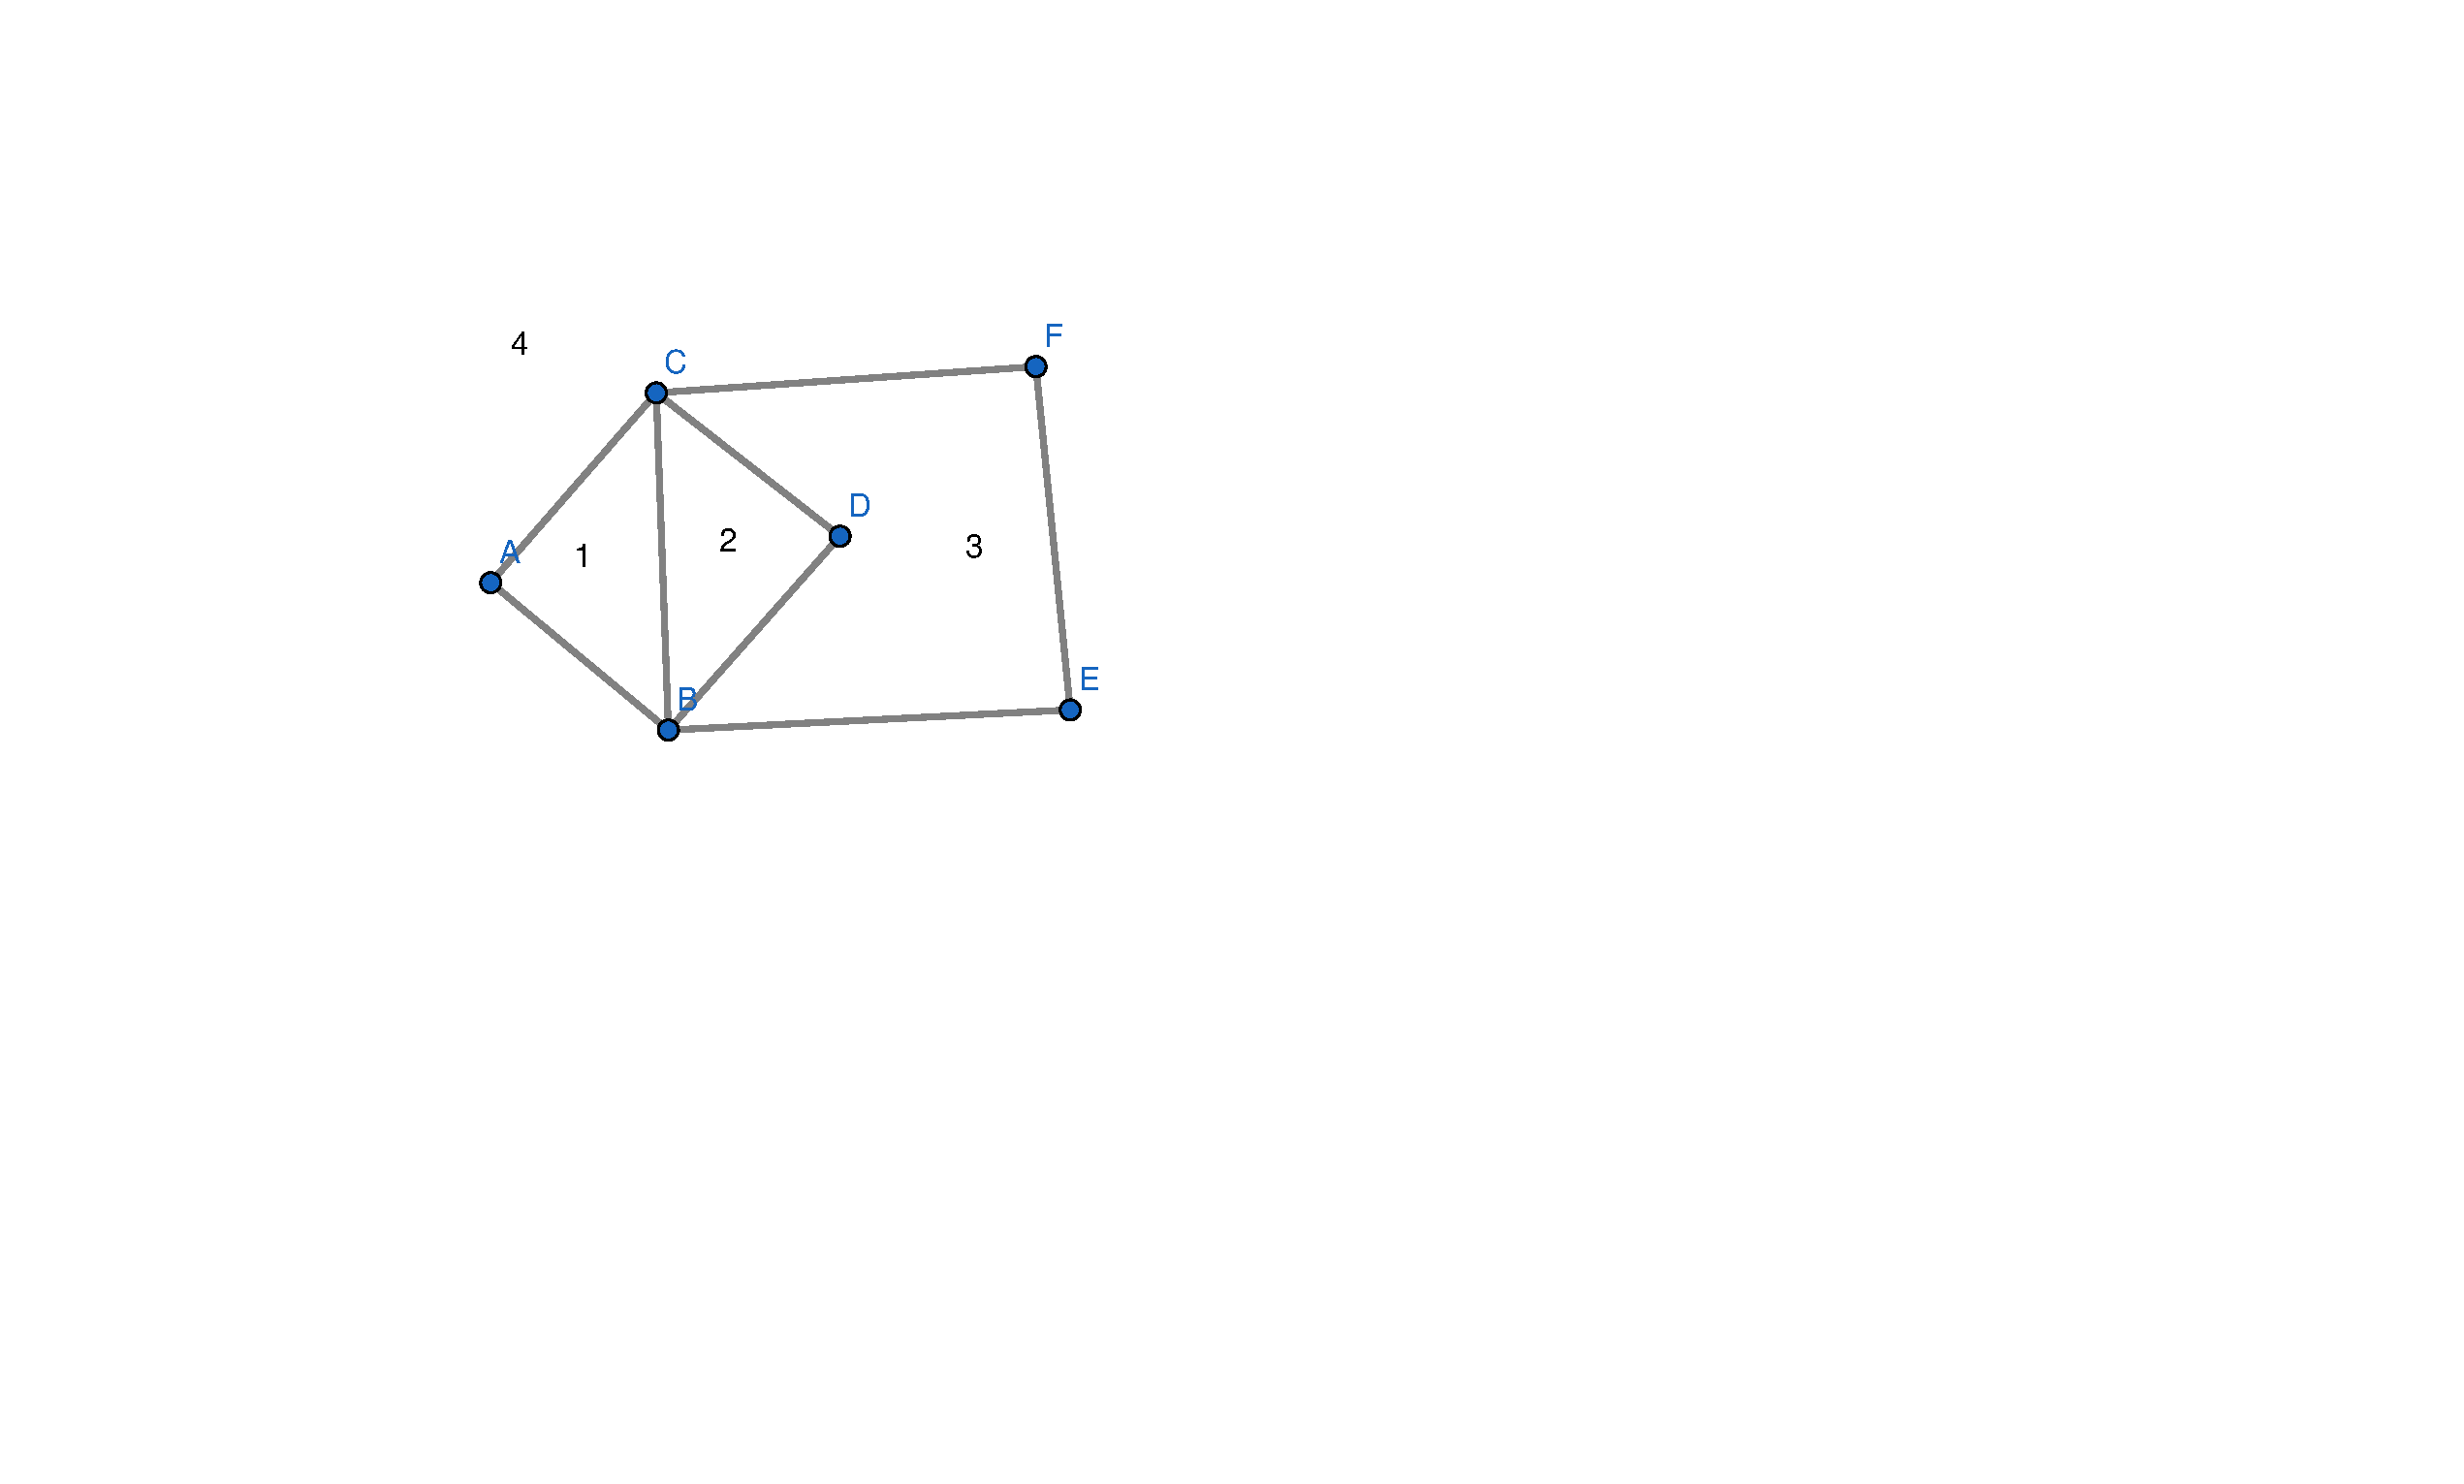
\includegraphics[width=15cm]{faces}
        \caption{Die Faces sind die Flächen, die durch die Kanten eingeschlossen werden.}
        \label{fig:}
    \end{center}
\end{figure}



\paragraph{Alternativ} Festlegung der Reihenfolge der Nachbarknotes jedes Knotens (Adjazenzliste) in einer möglichen planaren Zeichnung gegen den Uhrzeigersinn. Wir arbeiten meistens mit der 2. Alternative. Die beiden Definitionnen sind äquivalent.

\paragraph{Planaritätstest} bzw Einbettung besteht dann in der Aufgabe die Adjazenzlisten in eine Reihenfolge zu sortieren, so dass diese eine planare Einbettung definiert (falls möglich). Im Allgemeinen besitzt ein planarer Graph verschiedene panare Einbettungen (Hinweis: Einbettung ist eindeutig für 3-fach zusammenhängende Graphen). Beispiel für nicht-eindeutige Einbettungen (siehe Graphik). Die Faces sind die Flächen, die durch die Kanten eingeschlossen werden.

% Einbettung 
\begin{figure}[h]
    \begin{center}
        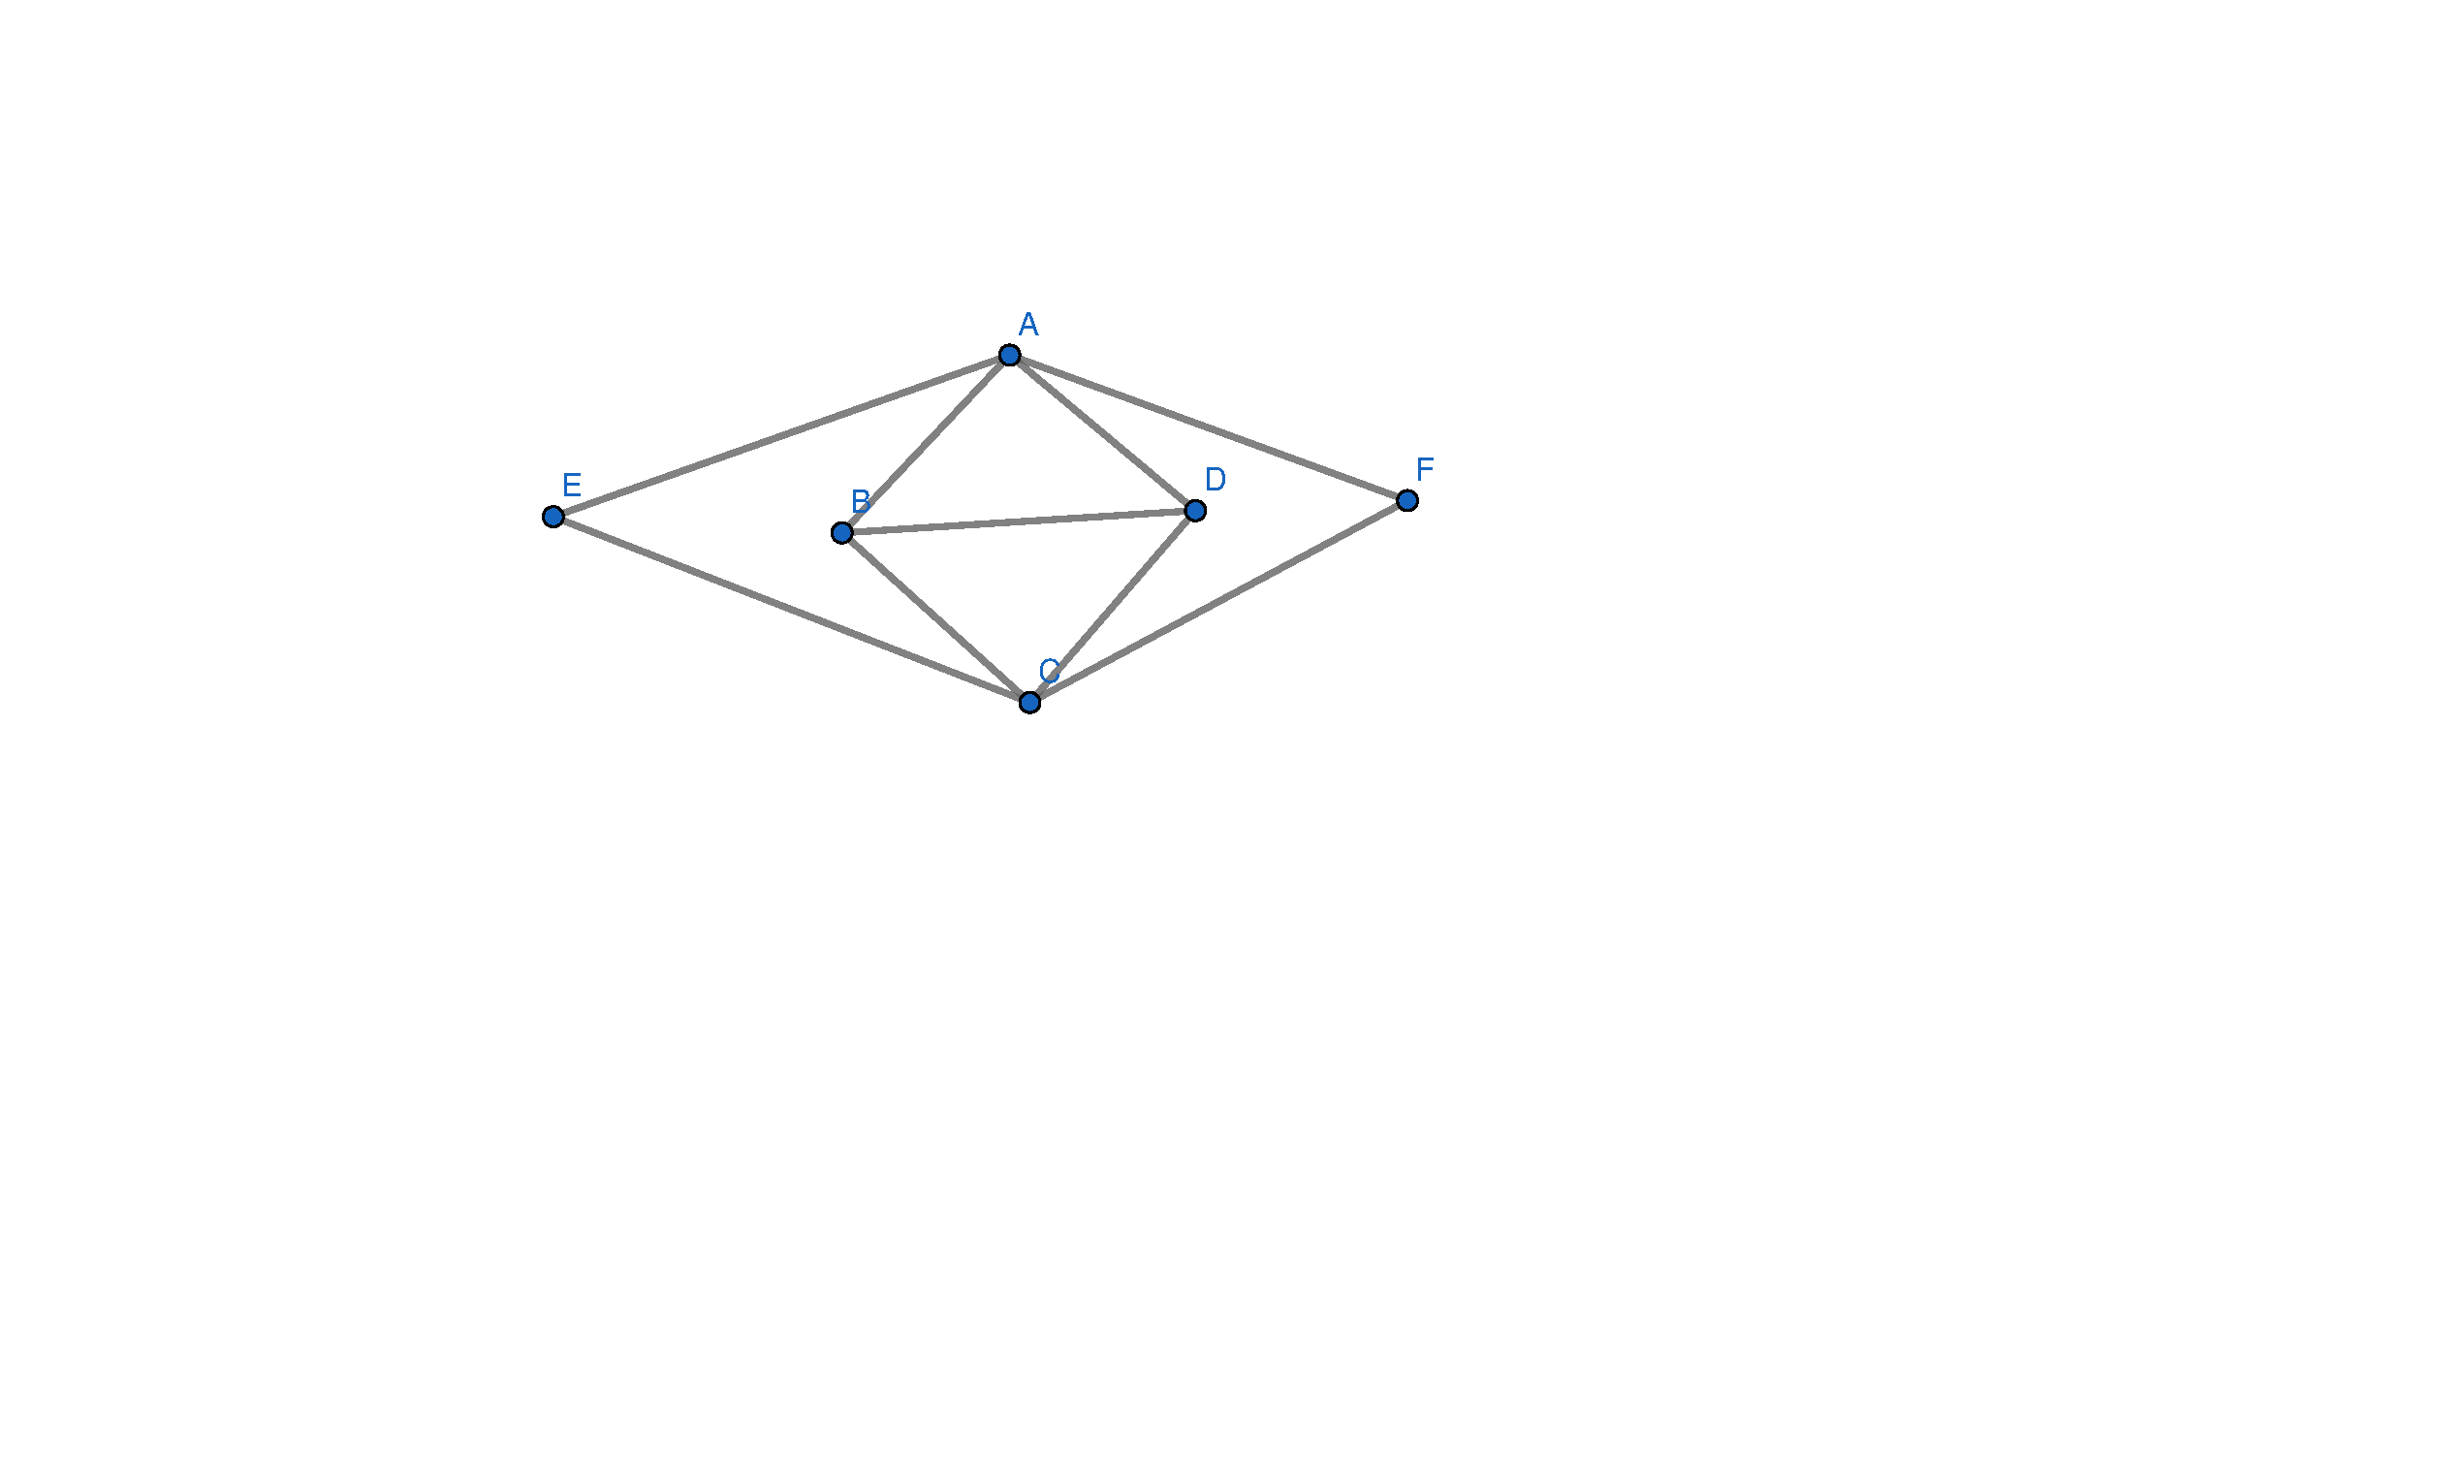
\includegraphics[width=15cm]{einbettung}
        \caption{Graph mit nichteindeutiger Einbettung: Rotation des unteren Teils (B und D)ergibt verschiedene Faces}
        \label{fig:}
    \end{center}
\end{figure}

\paragraph{Unterteilung (Subdivision)}
Sei G ein ungerichteter Graph. G' heißt Unterteilung oder Subdivision von G, wenn G' aus G durch ersetzen von Kanten durch Pfade entsteht (Platzieren neuer (Unterteilungs-)Knoten auf bestehende Kanten).

\subsection{Die Euler-Formel}
Sei G eine zusammenhängende planare Einbettung mit n Knoten, m Kanten und f Faces. Dann gilt
$$ n - m + f = 2 $$
\newpage
\begin{proof}[Beweis\ Euler-Formel]
Induktion über m\\
$\underline{m = 0:} $ Graph besteht aus einem isolierten Knoten: n=1, f=1  \\
$\underline{m > 0:} $ Sei G eine planare Einbettung mit m Kanten, n Knoten und f Faces \\
$\underline{IA} $ Für alle Einbettungen mit m-1 Kanten gilt die Formel \\
$\underline{Fall 1} $ G ist azyklisch (dh: Baum) 
\begin{enumerate}
    \item f = 1
    \item G besitzt Knoten v mit $ deg(v)=1 $ (Blatt)
\end{enumerate}
Die planare Einbettung $ G\backslash \{v\} $ ist zusammenhängend und hat n-1 Knoten und m-1 Kanten. 
$$ IA: (n-1) - (m-1) + f = 2 $$
$\underline{Fall 2} $ G ist kein Baum dh besitzt einen Kreis (f>1). Sei e eine beliebige Kante auf dem Kreis. Betrachte die planare Einbettung $ G\backslash \{e\} $

\begin{itemize}
    \item $ G\backslash \{e\} $ ist zusammenhängend
    \item $ G\backslash \{e\} $ hat m-1 Kanten, n Knoten und f-1 Flächen
\end{itemize}
$$ IA: n - (m-1) + (f - 1) = 2 $$

\end{proof}

\subsubsection{Folgerung}
Sei G ein planarer Graph mit $ n \geq 3 $ Knoten und m Kanten, dann gilt $ m = 3n-6 $. dh $ m=O(n) $, also linear viele Kanten.
\begin{proof}
Ein maximal planarer Graph ist ein planarer Graph, der durch Hinzufügen einer Kante $ (v,w) \notin E $ nicht-planar wird. Beobachtung: Alle Faces in jeder planaren Einbettung von G sind Dreiecke (Triangulierung). Jedes Face in einer Triangulierung hat 3 Rand-Kanten und jede Kante liegt am Rand von 3 Faces. 
$$\Rightarrow 3f = 2m $$
Einstetzen in Euler-Formel
$$ n - m + \frac{2}{3}m = 2$$
$$ m = 3n-6$$
$ m \leq 3n-6 $ für beliebige planare Graphen
\end{proof}

%Graphik triangulierung
\begin{figure}[h]
    \begin{center}
        \includegraphics[width=15cm]{triangulierung}
        \caption{Beispiel für maximal planaren Graphen}
        \label{fig:}
    \end{center}
\end{figure}


\subsubsection{Folgerung}
Sie G ein \textbf{bipartiter} planarer Graph Dann gilt $ m \leq 2n-4 $. Beweis: Keine Kreise ungerader Länge in bipartiten Graphen. Kleinstmögliche Fläche in einem bipartiten Graphen ist ein Viereck.

\subsubsection{Folgerung}
$ K_{3,3} $ und $ K_5 $ sind nicht planar. Jeder planare Graph besitzt einen Knoten v mit $ deg(v) \leq 5 $.
\begin{proof}
\underline{Annahme} $ \forall v \in V\ deg(v)\geq 6,\ m = \sum_{v\in V} \frac{deg(v)}{2} \geq \frac{6n}{2} = 3n$
\end{proof}

\subsection{Das Färbungsproblem für planare Graphen}
Knotenfärbung: k Farben $ \{1, ..., k \} $. Finde eine Abbildung $ f: \rightarrow \{1, ..., k \} $, sodass $ f(v) \neq f(w) $ für alle Kanten $ (v,w) \in E $. \textbf{Frage:} Wie viele Farben k sind notwendig? (minimales k):
\begin{itemize}
    \item k=n geht immer
    \item notwendig k=n für $ K_n $
\end{itemize}  
\subsubsection{Vierfarbensatz}
k=4 für planare Graphen. Ursprung in der Darstellung von Landkarten beim Einfärben der Länder, sodass benachbarte Länder verschiedene Farben haben.
\paragraph{Dualer Graph} $ G=(V,E) $ Für jedes Land (Fläche) einen Knoten $ v \in V, (v,w) \in E \Leftrightarrow $ Länder v und w haben eine gemeinsame Grenze.
\begin{enumerate}
    \item G ist planar
    \item Knotenfärbung von G $ \Leftrightarrow $ Färbung der Karte
\end{enumerate}
Einfacher, als der Vierfarbensatz ist der Fünffarbensatz.
\begin{proof}
Induktion über n \\
\underline{IA} für alle Grapfen mit $ n \leq 5 $. \\
Sei G ein planarer Graph mit $ n > 5 $. Aus Folgerung 3: G besitzt einen Knoten mit $ deg(v) \leq 5 $.\\
\underline{Fall 1} G besitzt einen Knoten v mit $ deg(v) \leq 4 $. Nach IA $ G \backslash \{ v \} $ besitzt eine 5-Färbung. Betrachte die r Farben den Nachbarn von v in G, dann gilt $ r \leq 4\ (deg(v) \leq 4) $ $ \Rightarrow $ mindestens eine Farbe frei. Diese erhält v. \\
\underline{Fall 2} Alle Knoten haben mindestens Grad 5. Aus Folgerung 3: Sei $ v\in V $ mit $ deg(v) = 5 $. Beobachtung: v besitzt 2 Nachbarnknoten x, y mit $ (x,y) \notin E $ (dh x,y unabhängig), sonst totaler Graph $ K_5 $. Betrachte $ G' = G\backslash\{v \} $: Planare Einbettung von G und entferne v. G'' = Veschmelze die unabhängigen Knoten x und y zu einem Knoten z. G'' ist planar. G'' hat nur noch n-2 Knoten.\\
Aus IA: G'' kann mit 5 Farben gefärbt werden. Sei c die Farbe von z in dieser Färbung. Expandiere Z wieder zu x, y mit $ color(x)=color(y)=c $. $ \Rightarrow $ Die 5 Nachbarn von v belegen höchstens 4 Farben und eine Farbe ist frei.
\end{proof}
\paragraph{Andere Anwendung} Finde eine große unabhängige Knotenmenge (Independent Set). Beobachtung: 5-Färbung $ \rightarrow $ Farbklasse  (Menge von Knoten der gleichen Farbe) mit mindestens $ \frac{n}{5} $ Knoten. Alle Knoten einer Farbe bilden ein Independent Set.


\subsection{Satz von Kuratowski}
\paragraph{Notation} Verschmelzung (Kontraktion) entlang einer Kante $ e=(v,w) $: $ G|e \rightarrow$ Graph den man durch Verschmelzen der Endknoten v und w. G planar $\Rightarrow G|e $ planar.
\paragraph{Satz} Ein Graph G ist genau dann planar, wenn er keine Unterteilung (Subdivision) des $ K_5 $ oder $ K_{3,3} $ enthält.

\begin{proof} Satz von Kuratowski \\
$ \Rightarrow $ trivial \\
$ \Leftarrow $ (Jeder Graph ohne eine Unterteilung des $ K_5 $ oder $ K_{3,3} $ ist planar) Induktion über n\\
Sei G ein Graph mit n Knoten, der keine Unterteilung des $ K_5 $ oder $ K_{3,3} $ enthält. \\
\underline{IB} $ n \leq 5 $ (dh, kein $ K_5 $)\\
\underline{IA} Für alle Graphen mit weniger als n Knoten gilt die Behauptung \\
\underline{Fall 1} G ist nicht 3-fach zusammenhängend \\
Angenommen, G ist 2-fach zusammenhängend$ \Rightarrow $ G bestitzt ein Separationspaar (x,y), das G in die Blöcke $ G_1 $ und $ G_2 $ zerlegt, mit jeweils weniger, als n. Offensichtlich enthalten $ G_1 $ und $ G_2 $ keinen $ K_5 $ oder $ K_{3,3} $. Nach IA sind $ G_1 $ und $ G_2 $ planar. Betrachte jeweils eine planare Einbettung von $ G_1 $ und $ G_2 $ mit x und y (bzw Kanze (x,y)) außen liegt. Dann kann man diese Eingbettungen leicht zu einer Einbettung von G zusammenfügen. $ \Rightarrow $ G ist planar. \\
\underline{Fall 2} G ist 3-fach zusammenhängend \\

\paragraph{Lemma 1} Die planare Einbettung aus 2-fach zusammenhängenden Graphen G ist eindeutig, genau dann wenn G eine Unterteilung eines 3-fach zusammenhängenden 
Graphen.

\paragraph{Corollar} Die planare Einbettung eines 3-fach zusammenhängenden Graphen ist eindeutig.

\paragraph{Lemma 2} Sei G ein 3-fach zusammenhängender Graph mit mindestens 5 Knoten. Dann enthält G eine Kante e, sodass $ G|e $ 3-fach zusammenhängend ist.

\paragraph{Lemma 3} Sei e eine beliebige Kante in G. Falls $ G|e $ eine Unterteilung des $ K_5 $ oder $ K_{3,3} $ enthält, dann gilt dies auch für G. Dh Kontraktion einer Kante erzeugt keinen $ K_5 $ oder $ K_{3,3} $.\\
\underline{IS} Sei G ein 3-fach zusammenhängender Graph mit n Knoten ohne $ K_5 $ oder $ K_{3,3} $. Aus Lemma 2 folgt $ \exists $ Kante e, sodass $ G|e $ (=G') 3-fach zusammenhängend ist. Aus Lemma 3 folgt G' hat weder $ K_5 $ noch $ K_{3,3} $. Nach IA ist G' planar. Aus Lemma 1 folgt, G' hat eine eindeutige planare Einbettung. Betrachte diese Einbettung in der Umgebung von z (=Knoten, der aus der Knotraktion von x,y entsteht). Seien $ x_1, ..., x_k $ die Nachbarknoten von z, angeordnet im Uhrzeigersinn, gemäß der planaren Einbettung. Ersetze z wieder durch die Kante (x,y) und Konstruiere eine planare Einbettung für G. Sei $ x'_1, ... , x'_l $ die Teilfolge der Knoten $ x_1, ..., x_k $, die in G benachbart zu x sind. \\
\underline{Fall 1} Alle Nachbarn von y liegen auf einem Face-Segment zwischen $ x'_i $ und $ x'_{i+1} $ zyklisch und inklusive Ränder. $ deg(y) \geq 3 $, da G 3-fach zusammenhängend. Dann kann man leicht eine planare Einbettung für G' konstruieren. \\
\underline{Fall 2} Nicht alle Nachbarn von y (außer x) liegen im selben Segment ($ x'_i $, $ x'_{i+1} $) \\
\underline{Fall 2.1} y hat $ \geq $ 3 Nachbarn in $ x'_1, ... , x'_l $. G enthält eine Unterteilung des $ K_5 $ definiert durch die Kanten.

% Graphik Fall 2.1
\begin{figure}[h!]
    \begin{center}
        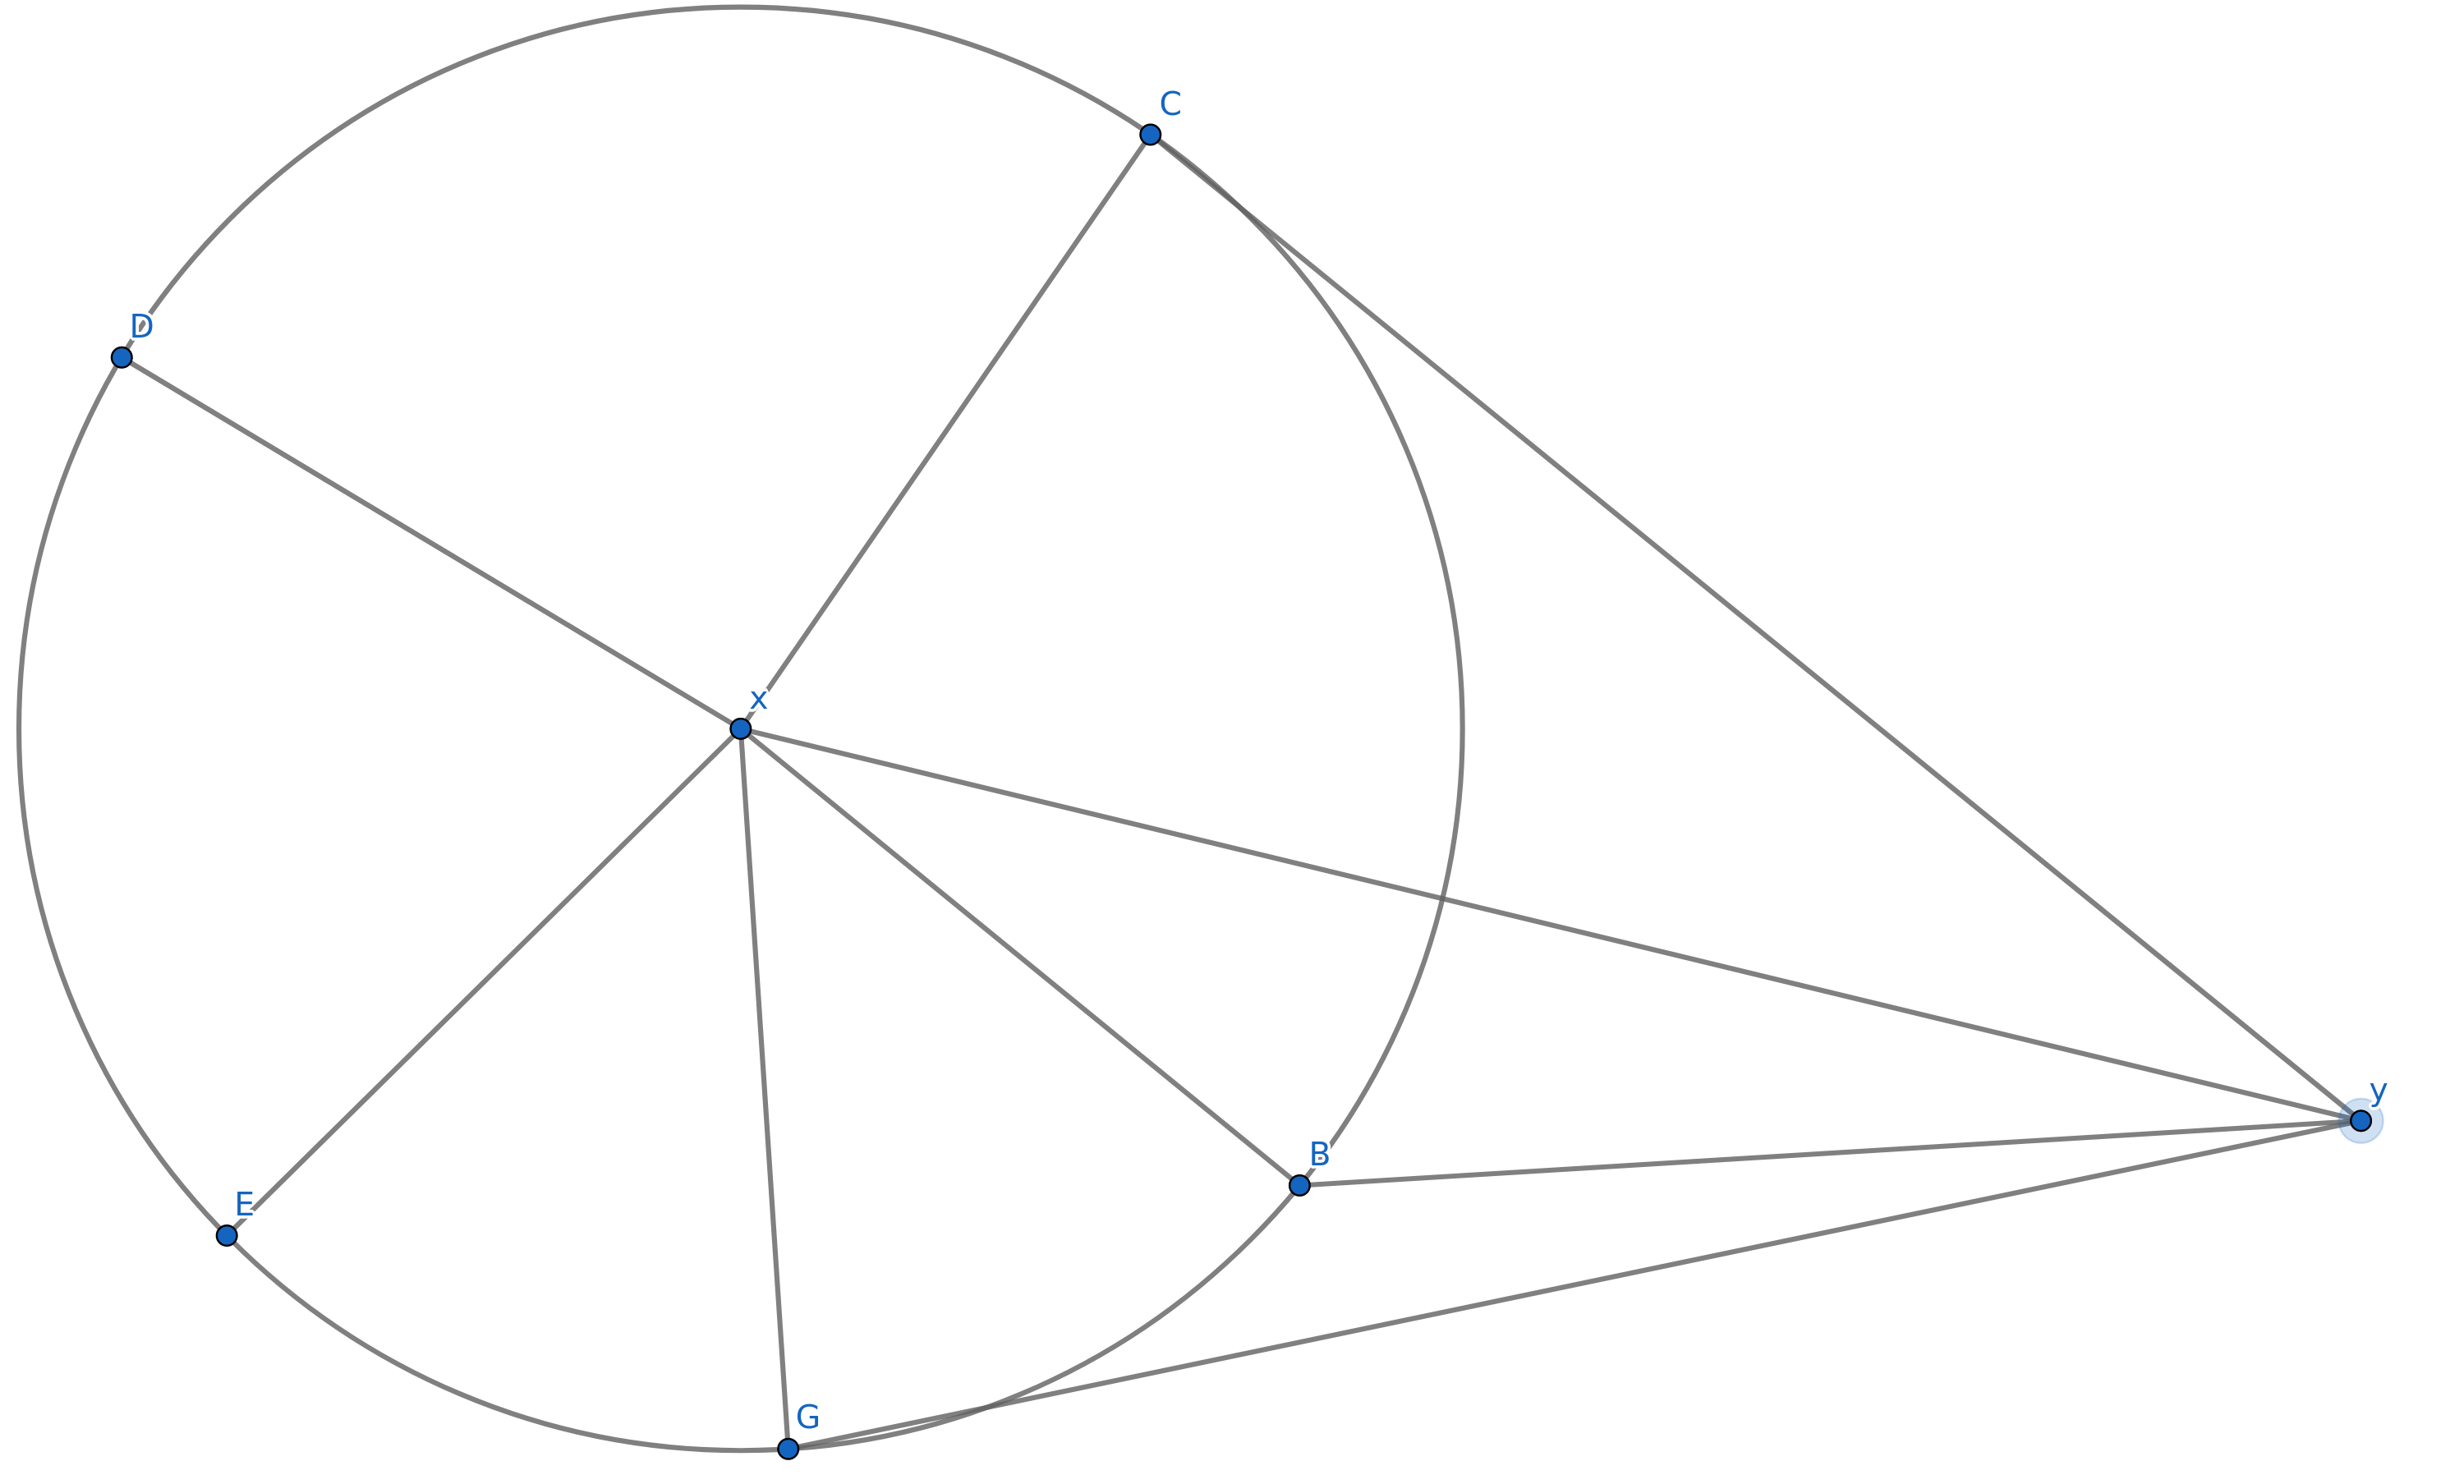
\includegraphics[width=10cm]{fall21}
        \caption{Beweis Satz von Kuratowski: Fall 2.1}
        \label{fig:}
    \end{center}
    \begin{center}
        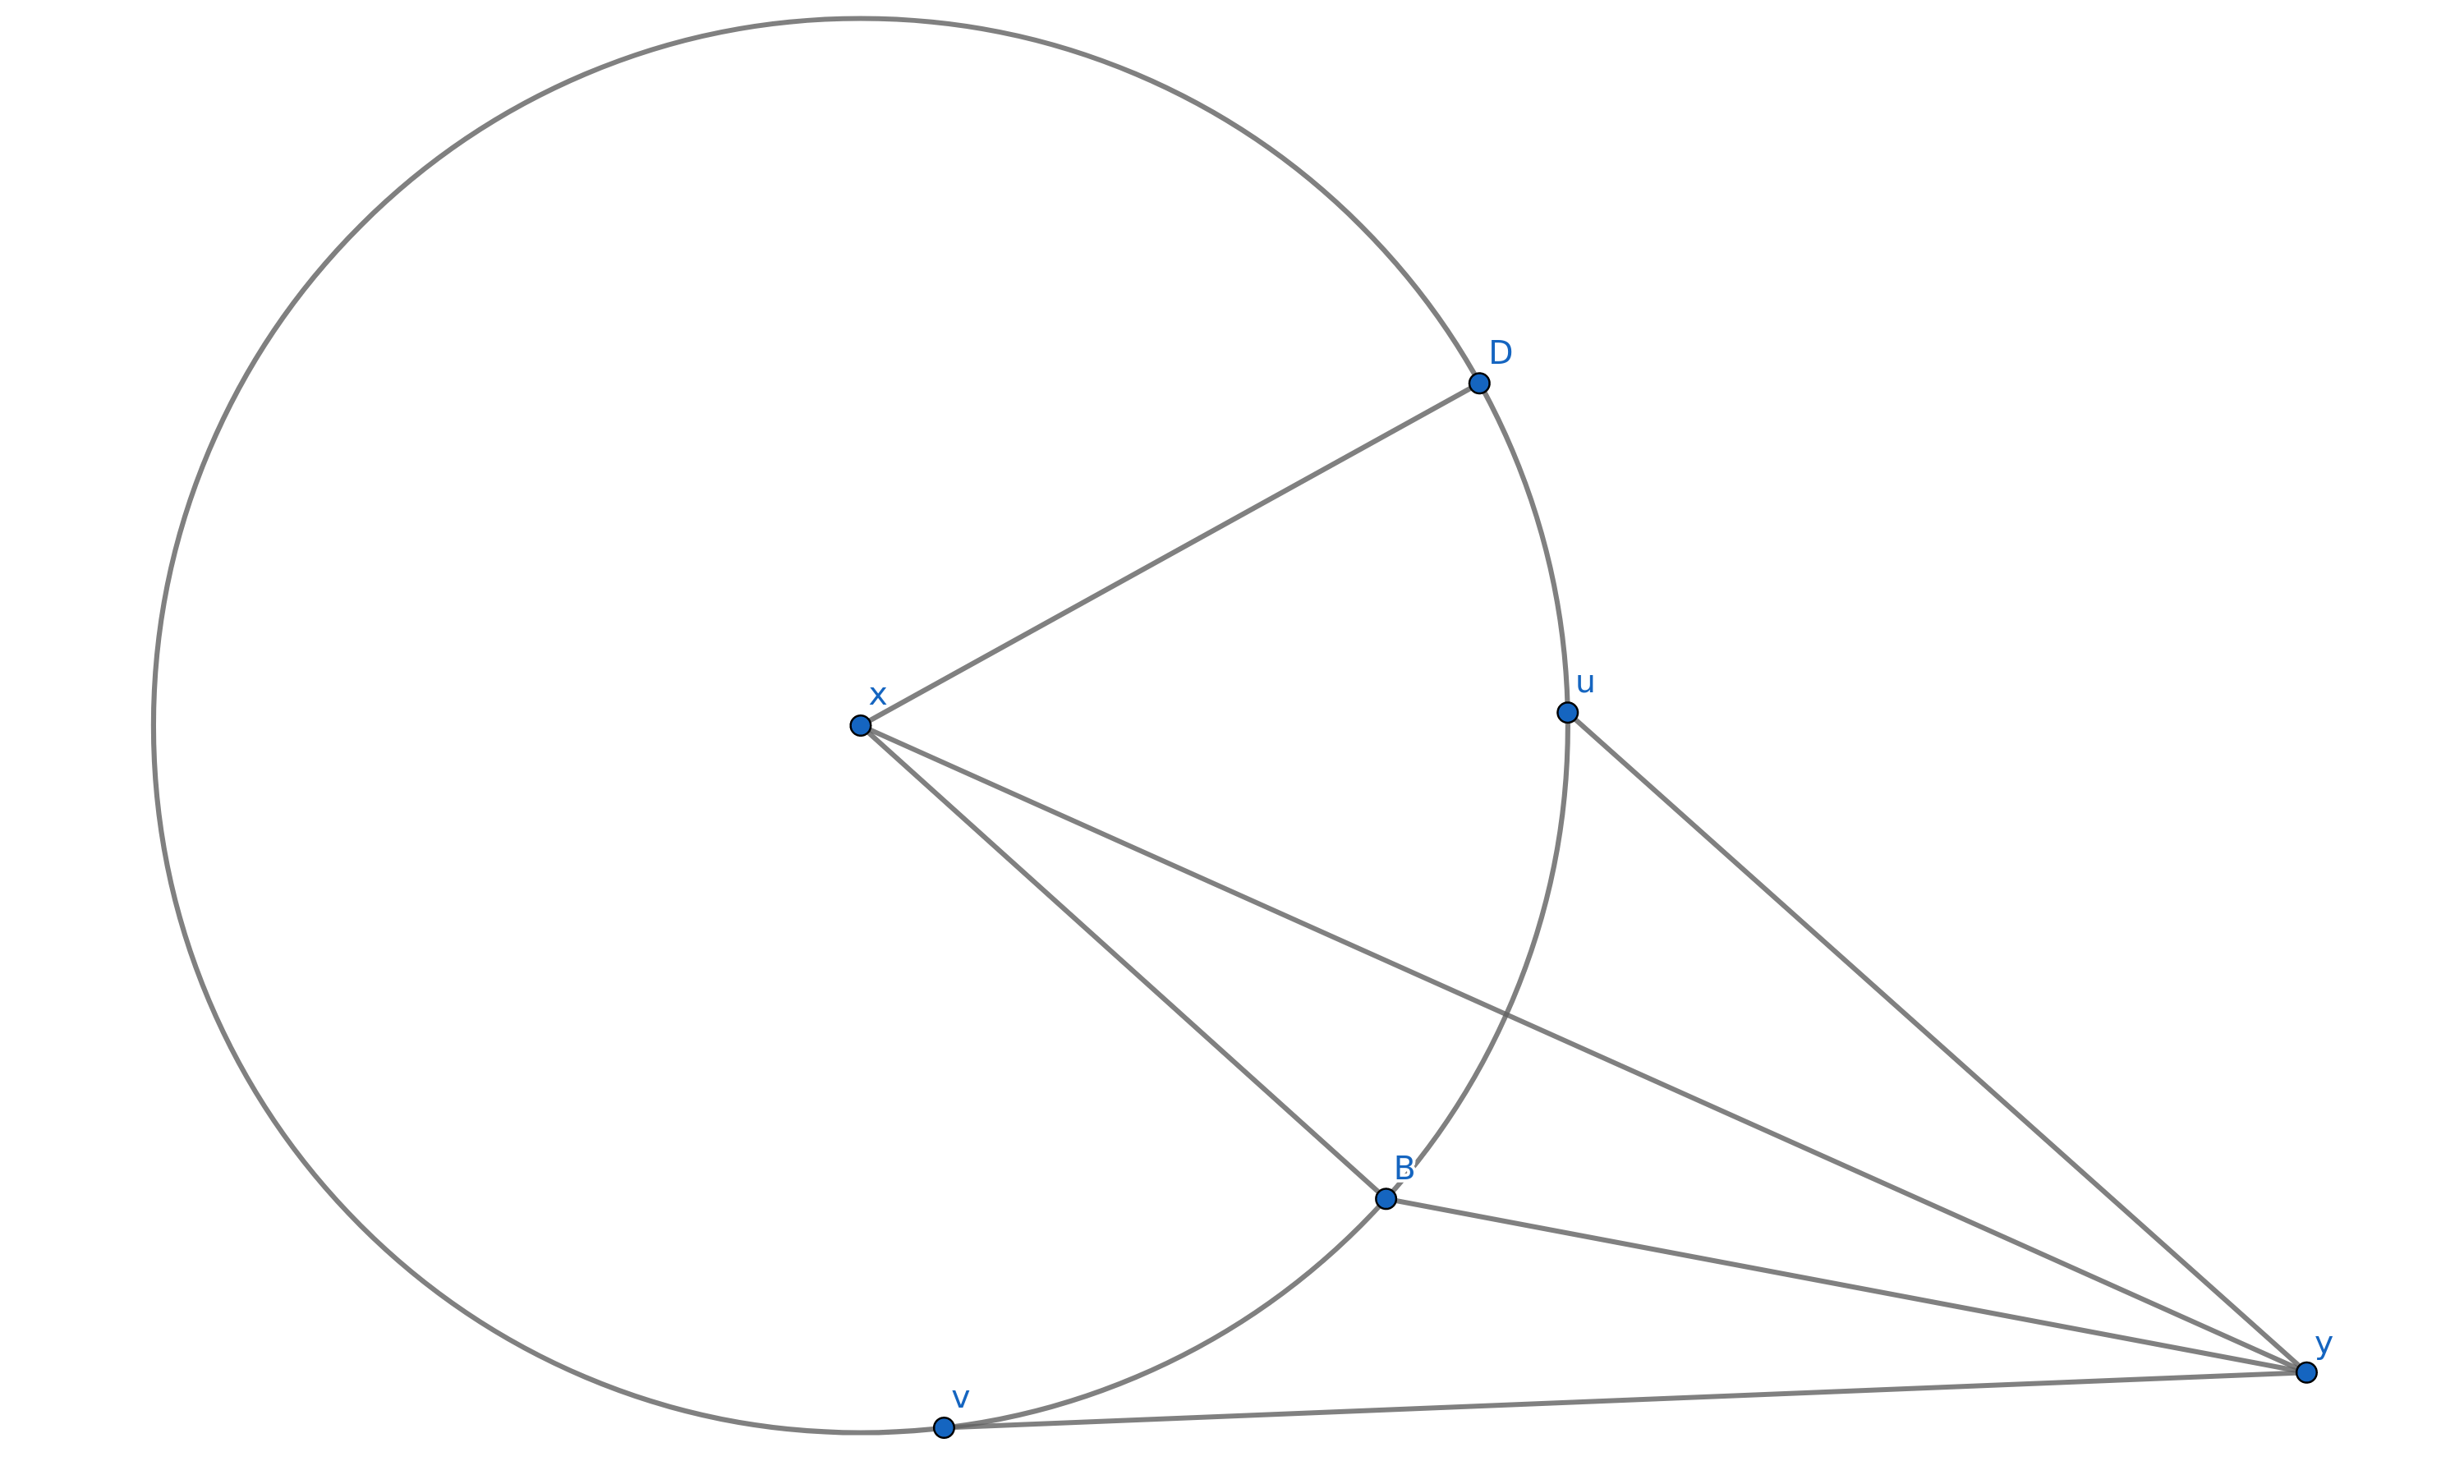
\includegraphics[width=10cm]{fall22}
        \caption{Beweis Satz von Kuratowski: Fall 2.2}
        \label{fig:}
    \end{center}
    \begin{center}
        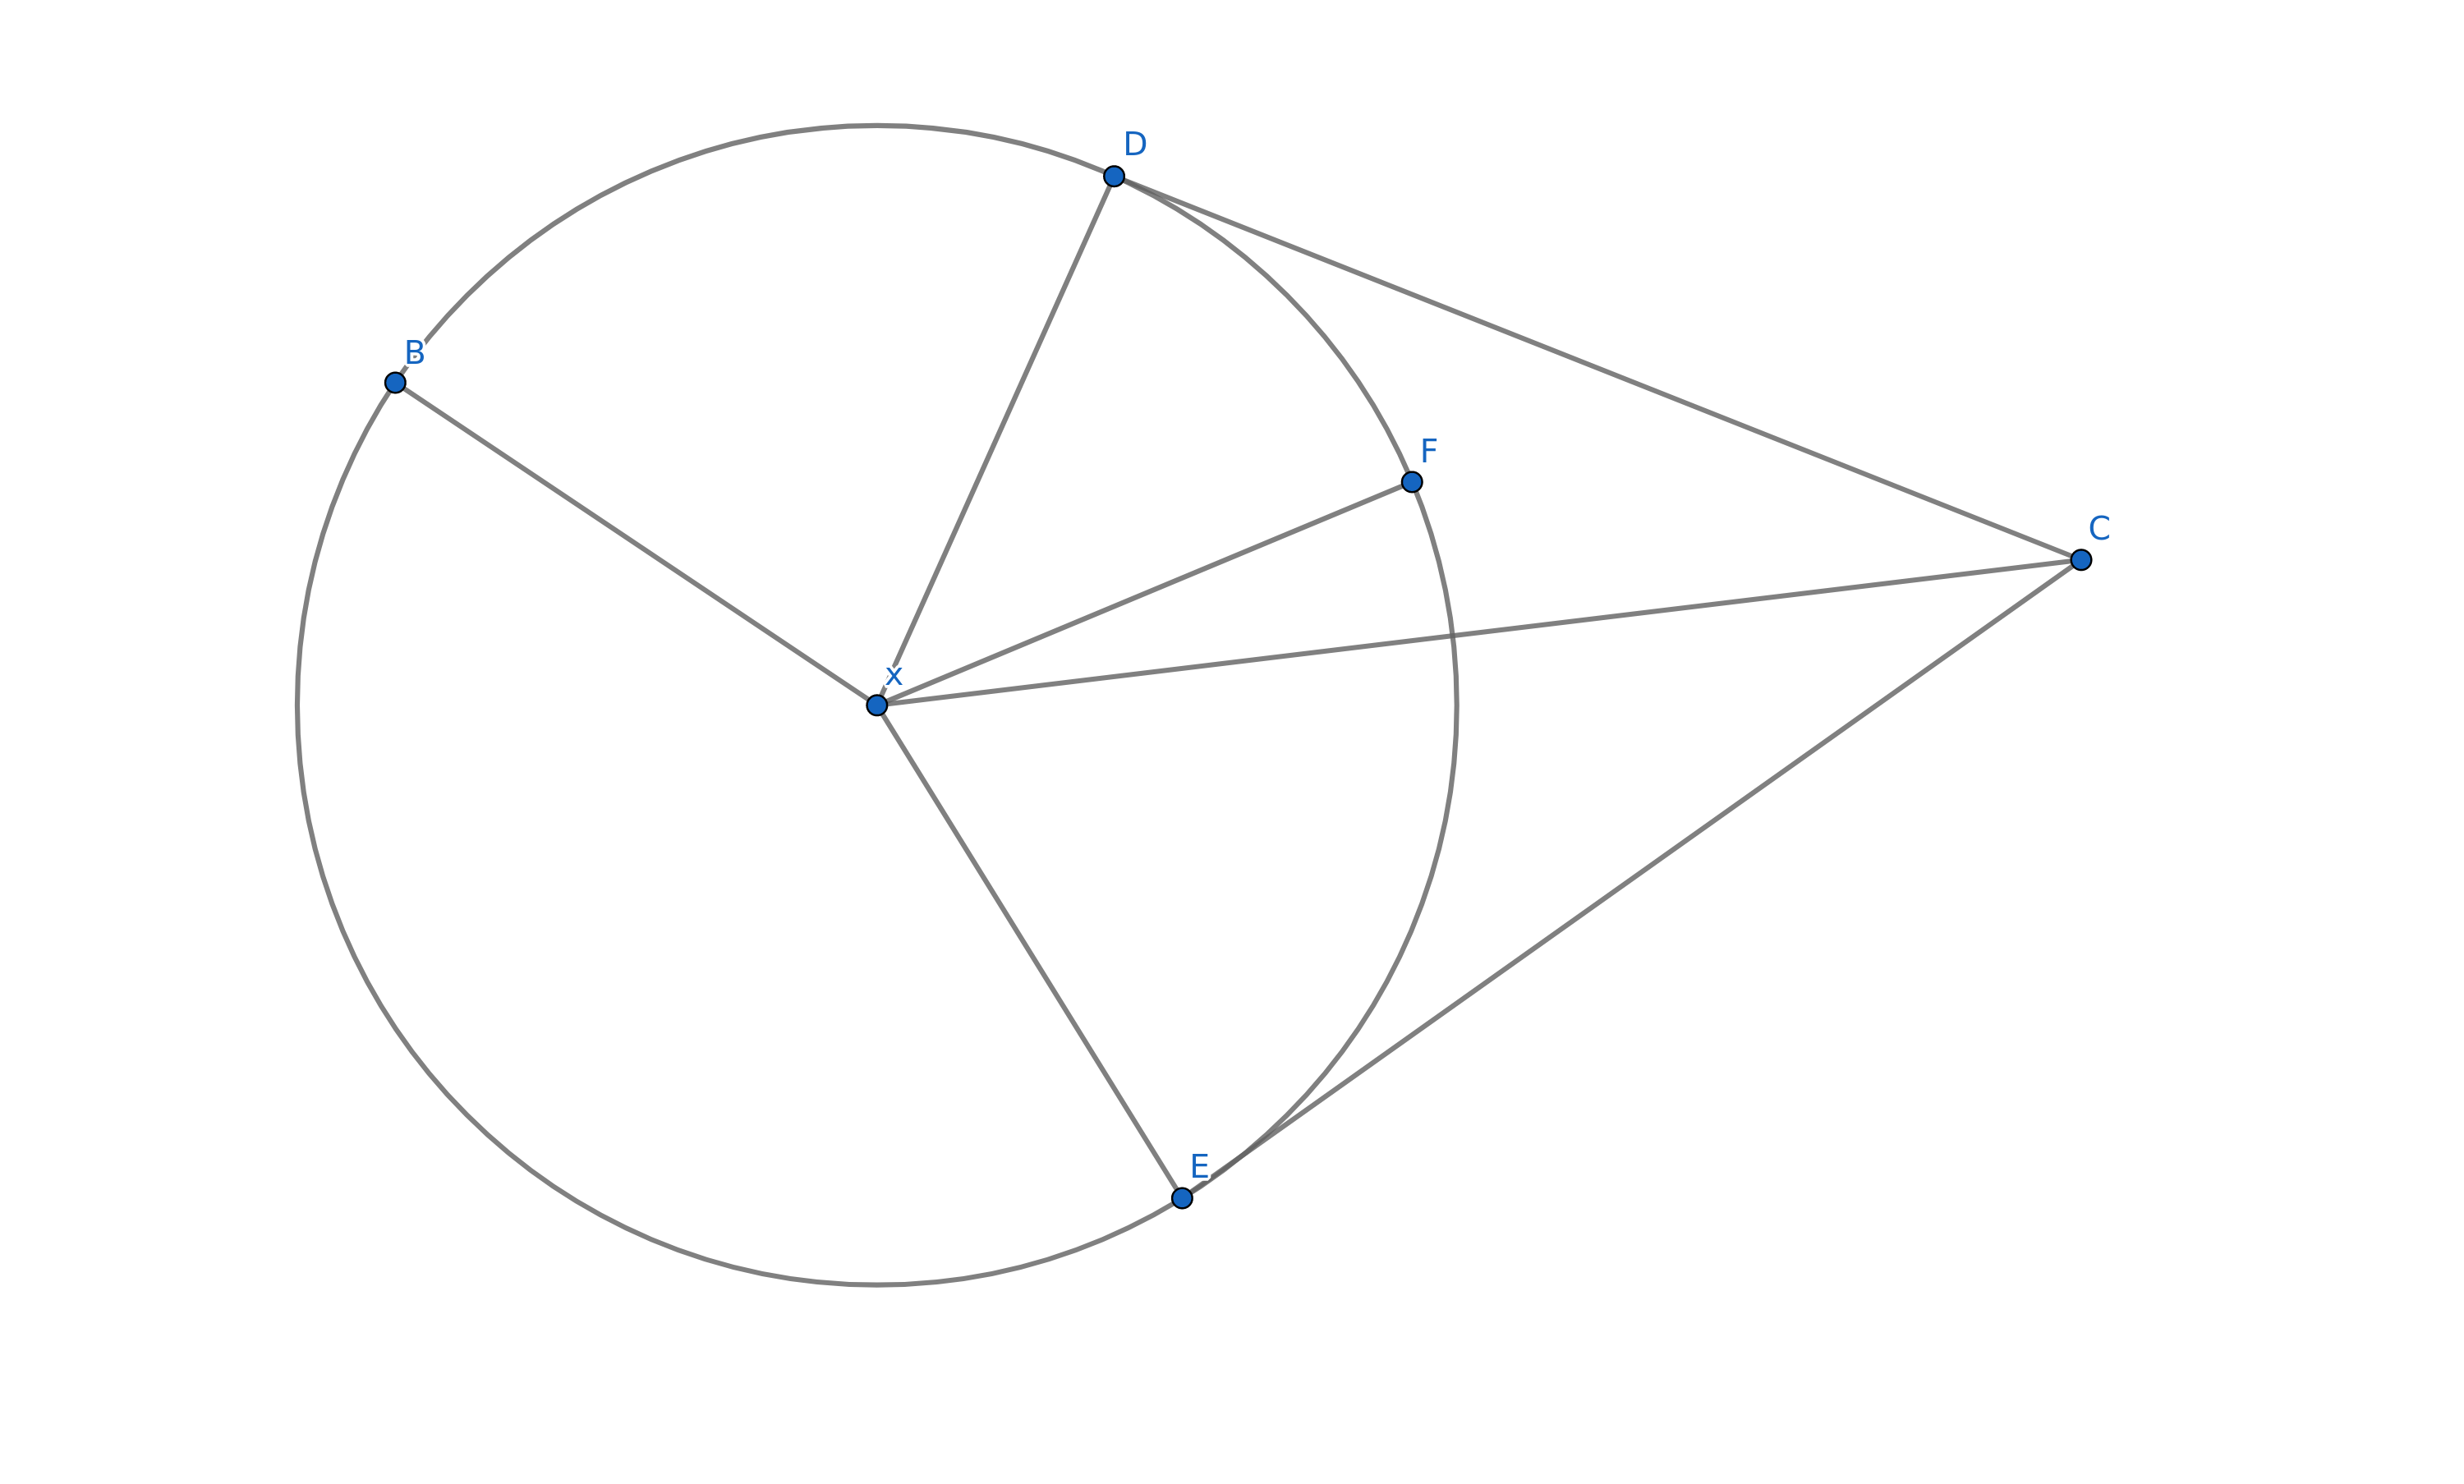
\includegraphics[width=10cm]{fall23}
        \caption{Beweis Satz von Kuratowski: Fall 2.3}
        \label{fig:}
    \end{center}
\end{figure}

\underline{Fall 2.2} y hat  einen Nachbarn u in einem Segment $ P_i = (x'_i, x'_{i+1}) \backslash(x'_i, x'_{i+1}) $ und einem anderen u $ \notin P_i $. 
G enthält eine Unterteilung des $ K_{3,3} $


\underline{Fall 2.3} y hat 2 Nachbarn in $ x'_1$ und $ x'_j $ mit $ j \neq i+1 $ und $ i \neq j+1 $ (zyklisch). G enthält eine Unterteilung des $ K_{3,3} $

$ \Rightarrow $ Es kann nur Fall 1 vorkommen, also ist G planar. 
\end{proof}

\subsubsection{Beweise der Lemmata}

\paragraph{Lemma 1} Die Einbettung eines zweifach planaren Graphen G ist eindeutig $ \Leftrightarrow $ G ist eine Unterteilung eines 3-fach zusammenhängenden Graphen.

\begin{proof}
Für A $ \Leftrightarrow $ B zeige:
\begin{enumerate}
    \item $ \overline{B}  \Rightarrow \overline{A}$
    \item $ \overline{A}  \Rightarrow \overline{B}$
\end{enumerate}

\paragraph{1)} Sei G 2-fach zusammenhängend, aber keine Unterteilung eines 3-fach zusammenhängenden Graphen. \underline{Beobachtung} Dann existiert ein Separationspaar x, y mit Split-Graphen $ G_1 $ und $ G_2 $, sodass weder $ G_1 $ noch $ G_2 $ ein Pfad ist. \underline{Annahme} Für alle Separationspaare (x,y) sind diese Splitgraphen Pfade $ \Rightarrow $ G ist eine Unterteilung eines 3-fach zusammenhängenden Graphen \textbf{Widerspruch zur Annahme}. Betrachte eine planare Einbettung von G und das Separationspaar (x, y) gemäß Beobachtung. Durch Drehung bzw Spiegelung von $ G_1 $ oder $ G_2 $ in dieser Einbettung erhält man eine neue Einbettung. Ist nur eine Seite eine Pfad, existiert nur eine Einbettung.
\paragraph{2)} Sei G 2-fach zusammenhängend und planar mit einer nicht-eindeutigen Einbettung. Dh, es existieren mindestens 2 verschiedene Einbettungen E(G) und E'(G). $ \Rightarrow $ es existiert ein Face Zyklus C in E, der nicht in E' existiert. Betrachte E mit C als äußeres Face. C zerlegt G in mindestens 2 Komponenten, die wahlweise auf der einen oder anderen Seite von C eingebetter werden können. Dann existieren 2 Knoten x,y auf C die die beiden Komponenten trennt. $ \Rightarrow $ (x,y) ist ein Separationspaar, sodass beide Split-Graphen keine Pfade sind. $ \Rightarrow $ G ist keine Unterteilung eines 3-fach zusammenhängenden Graphen.
\end{proof}

\paragraph{Lemma 2} Sein G ein 3-fach zusammenhängender Graph mit mindestens 5 Knoten, dann existiert eine Kante e in G, sodass $ G|e $ 3-fach zusammenhängend ist.

\begin{proof}(indirekt) \\
\underline{Annahme} Für jede Kante e in G: $ G|e $ ist nicht 3-fach zusammenhängend. $ \Rightarrow $ $ G|e $ enthält ein Separationspaar (x', z). Sei e=(x,y) mit x' als Resultat der Kontraktion von (x,y), Im Originalgraphen G ist $ \{x,y,z \} $ eine Separationsmenge. Wähle die Kante e=(x,y) und den Knoten z so, dass eine möglichst große Komponente Komponente H entsteht. Sei H' der Rest der Grpahen (ohne H, x, y, z). Dann betrachte eine Kante e'=(z,v) mit u in H' (existiert, denn sonst wäre (x,y) ein Sep-Paarin G). Auch $ G|e' $ ist nicht 3-fach zusammenhängend (nach Annahme) $ \Rightarrow $ Es existiert ein Knoten v mit  $ \{x,y,z \} $ ist Separationsmenge von G. Für v gibt es 3 Möglichkeiten:
\begin{enumerate}
    \item $ v \in H' $
    \item v = x. Dann existiert Komponente, die mindestens H und y enthält. Widersprch zur Maximalität con H.
    \item v = y. Symmetrisch zu Fall 2 (Widerspruch)
\end{enumerate}
Das sind alle möglichen Fälle. Dh $ v \notin H $

\paragraph{3} Für jede Kante e: $ G|e $ enthält eine Unterteilung des $ K_5 $ oder $ K_{3,3} $ $ \Rightarrow $ G enhält eine solche Unterteilung. 

\end{proof}

\section{Maximal Matchings im bipartiten Graphen}

\paragraph{Definition} Sei G = (V, E) ein ungerichteter Graph
\begin{enumerate}
    \item $ M \subseteq E $ heißt Matching von G, falls keine 2 Kanten aus M einen gemeinensamen Endpunkt (Knoten) haben.
    \item Falls $ e \in M $, dann heißt e paarned. Ein Knoten v heißt gepaart, falls er einen Endpunkt einer paarenden Kante ist.
    \item Ein Matching M heißt maximal, falls $ |M| \geq |M'| $ für alle Matchings M'. 
\end{enumerate}

\paragraph{Beobachtung} $ |M| \leq \lfloor \frac{n}{2} \rfloor \Rightarrow$ Falls $ M = \lfloor \frac{n}{2} \rfloor $, dann ist M maximal.

\paragraph{Idee für Algorithmus} Konstruiere $ M_i,...,M_l $ von Matchings mit $ |M_i| < |M_{i+1}| $ und $ M_l $ maximal. Schritt (Erhöhung/Erweiterung) $ M \rightarrow M' $ mit $ |M'| = |M| + 1 $.

\paragraph{Definition} Ein einfacher Pfad $ P = (v_1, v_2), (v_2, v_3), ..., (v_{2k-1}, v_{2k}) $ (ungerade Zahl von Kanten) heißt erweiternder Pfad (augmenting path) für ein Matching M, falls 
\begin{enumerate}
    \item $ v_1 $ und $ v_2 $ sind frei ($ \Rightarrow (v_1, v_2), (v_{2k-1}, v_{2k}) \notin M$)
    \item Kanten von P sind abwechselnd in M und $ E\backslash M $
\end{enumerate}
Beobachtung: Man kann M um 1 vergrößern durch vertauschen von paarenden und nicht paarenden Kanten von P. Für $ M = \emptyset $ gilt jede Kante (v,w) ist erhöhender Pfad. 

\subsection{Lemma 1} Sei M ein Matching und P ein erweiternder Pfad für M, dann ist $ M \oplus P = (M \cup P) \backslash (M \cap P) $ (symmetrische Differenz) ein Matching und $ |M \oplus P| = |M| + 1 $. 

\begin{algorithm}[H]
\SetAlgoLined
M $ \gets \emptyset $\;
 \While{$ \exists $ ein Pfad P für M  }{
    $ M \gets M \oplus P $\;
 }
 \caption{Grundalgorithmus }
\end{algorithm}
Beobachtung: Knotendusjunkte erweiternde Pfade $ P_1,...,P_k $ kommen gelichzeitig behandelt werden: $ M\gets M \oplus (P_1 \oplus P_2 \oplus ... \oplus P_H $. Problem: Finde möglichst viele Knotendisjunkte Pfade für ein Matching M in einem Schritt.

\subsubsection{Satz 1} Seien M und N Matchings mit $ |M| = r $ und $ |N| = s $ und $  s > r $. Dann enhält $ M \oplus N  $ mindestens s-r Knotendisjunkte erweiternde Pfade für M.

\begin{proof}

$ M \oplus N = (M\backslash N ) \cup (N \backslash M) $ dh Kanten die entweder in M oder in N sind. Sei $ \overline{G} = (V, M \oplus N) $. Da M und N Matchings sind, ist jeder Knoten in $ \overline{G}$ Endpunkt höchstens einer Kante aus $ M \backslash N $ und höchstens einer Kante aus $ M \backslash n $ $ \Rightarrow $ Für alle Knoten in $ \overline{G} $ gilt, $ outdeg_{\overline{G}}(c) \leq 2 $ dh $ outdeg_{\overline{G}}(c) \in \{1, 2, 3\} $ $ \Rightarrow  \overline{G}$ zerfällt in Zusammenhangskomponenten der folgenden Form
\begin{enumerate}
    \item isolierter Knoten
    \item Pfade, die abwechselnd Kanten aus $ M \backslash N $ und $ N \backslash N  $ enthalten.
    \item Kreis wie 2). 
\end{enumerate} 
\paragraph{Korollar 1} M ist maximales Matching $ \Leftrightarrow $ es existiert kein erweiternder Pfad für M
\end{proof}

\paragraph{Lemma 2} Sei M ein Matching mit $ |M| = r $ und $ s $ die Größes eines maximalen Matchings mit $ s>r $ (dh M ist nicht maximal). Dann gibt es für M einen erweiternden Pfad der Länge $ \leq 2 \cdot \lfloor \frac{r}{s-r} \rfloor + 1$.

\begin{proof}
Sie N ein max Matching ($ |N| = s $) \\
Aus Satz 1 $ \Rightarrow M \oplus N$ enthält mindestends s-r Knotendisjunkte erweiternde Pfade für M. Alle diese Pfade enthalten Zusammen $ \leq r $ Kanten aus M (da $ |M| = r $).\\
Verteile r Dinge auf s-r Pfade 

\begin{itemize}
    \item[] $ \Rightarrow \exists$ ein Pfad mit $ \leq \lfloor \frac{r}{s-r} \rfloor$ Kanten aus M 
    \item[] $ \Rightarrow \exists$ ein Pfad P mit  $|P| \leq 2 \cdot \lfloor \frac{r}{s-r} \rfloor + 1$
\end{itemize}
\end{proof}
 Ein erweiternder Pfad P für M heißt kürzester erweiternder Pfad, falls $ |P| \leq |P'| $ für alle erweiternden Pfade P' für M.

\subsubsection{Satz 2}
Sei M ein Matching, P ein kürzester erweiternder Pfad für M und P' ein beliebiger erweiternder Pfad für $ M \oplus P $. Dann gilt 
$$ |P'| \geq |P| + |P \cap P'| $$


\begin{proof} Satz 2 \\
$ M \rightarrow_P M \oplus P \rightarrow_{P'} \underbrace{M \oplus P \oplus P'}_N $. N ist ein Matching, $|N| = |M| + 2$. Aus Satz 1 $ \Rightarrow M \oplus N $ enthält 2 Knotendisjunkte erweiternde Pfade $ P_1,P_2 $ für M. 
$$ M \oplus N = M \oplus M \oplus P \oplus P' = P \oplus P ' $$
$$ \Rightarrow |P \oplus P'| = |M \oplus N | \geq |P_1| + |P_2| $$
Außerdem $ |P_1| \geq P, |P_2| \geq P $, da P ein kürzester erweiternder Pfad für M ist.
$$ \Rightarrow \underbrace{|P \oplus P'|}_{= |P| + |P'| - |P \cap P'| \geq 2 \cdot |P| } \geq |P_1| + |P_2| \geq 2 \cdot |P| $$
$$ \Rightarrow |P'| \geq |P| + |P \cap P'| $$

\end{proof}
 
\subsubsection{Neue Idee für Algorithmus} Berechne Folge von Matchings $ M_0, M_1,..., M_i $ mit 
\begin{enumerate}
    \item $ M_0 = \emptyset $
    \item $ M_{i+1} \gets M_i \cdot P_i $ mit $P_i$ ist ein erweiternder Pfad für $ M_i $
\end{enumerate}

\paragraph{Korollar 2} $ |P_i| \leq |P_{i + 1}| $, dh die Länge der kürzesten erweiternden Pfade ist in der Folge $ P_0,P_1,... $ monoton wachsend

\paragraph{Korollar 3} Für alle i,j mit $ i \neq j $ und $ |P_i| = |P_j| $ gilt $ P_i, P_j $ sind knotendisjunkt.


\subsubsection{Maximal Cardinality Matching Algorithmus}
Situation: Folge der kürzesten erhöhenden Pfade: $ \underbrace{P_0,P_1}_{\text{Abschnitte gleicher Länge}},\underbrace{...,...},\underbrace{...,P_s}$ (Abschnitt = Phase des Algorithmus)
\begin{enumerate}
    \item In jedem Abschnitt sind die Pfade knotendisjunkt
    \item Anzahl der Abschnitte $ \leq 2 \lfloor \sqrt{s} \rfloor + 2 $, dh $ s=O(\sqrt{n}) $
\end{enumerate}
Effizienter Algorithmus:
\begin{enumerate}
    \item Behandlung aller Pfade in einem Abschnitt (einer Phase) in Zeit $ O(n+m) $
    \item Das muss für $ O(\sqrt{n}) $ Abschnitte gemacht werden
    \item[] $ \rightarrow $ Laufzeit $ O(\sqrt{n} nm)= O(\sqrt{n} m)  (m \leq n) = O(n^{2,5} (m \leq n^2))$
\end{enumerate}
Im Gegensatz zum trivialen Algorithmus, der jeden Pfad getrennt durch Exploration des Graphen (Tiefen oder Breitensuche) betrachtet. Das führt zu einer Laufzeit von $ O(s(n+m)) = O(nm) = O(n^3)$ \\

Zwei Knotenmengen A, B (Seiten des Graphen). Darstellung eines Matchings M in bipartiten Graphen: \\
Idee $ \rightarrow $ gerichteter Graph.
\begin{itemize}
    \item[] Falls $ (v,w) \in M $, dann Richtung von B nach A
    \item[] Falls $ (v,w) \in M $, dann Richtung von A nach B
\end{itemize}
\paragraph{Beobachtung} (in der gerichteten Darstellung): Ein Pfad P ist genau dann ein ehöhender Pfad, wenn er in einem freien Knoten von A startet und in einem freien Knoten von B endet.

\paragraph{Erhöhung} $ M \oplus P $ in der Darstellung:
\begin{enumerate}
    \item Drehe alle Kanten von P um
    \item Endpunkte als gepaar markieren (nicht mehr frei)
\end{enumerate}

\paragraph{Algorithmus} sucht nach maximal vielen kürzesten erhöhenden Pfaden (gleicher Länge) und dreht alle Kanten dieser Pfade um. Wichtig dafür: Pfade sind Knotendisjunkt. Wiederhole, bis keine Pfade mehr existieren. \\

Kürzeste Pfade: Teile den Graphen in Schichten ein (Levels) ein.
\begin{itemize}
    \item[] Level 1: alle freien Knoten in A
    \item[] Level 2: alle von Level 1 über eine Kante erreichbar
    \item[] Level i: alle von Level i-1 über eine Kante erreichbaren, die nicht in Level i...i-1 enthalten sind.
    \item[] $ \Rightarrow $ Level i $ \subseteq $ A, falls i ungerade, Level i $ \subseteq $ B, falls i gerade.
\end{itemize}
Konstruiere den geschichteten Graphen $ \overline{G} $
\begin{enumerate}
    \item füge 2 Knoten s,t hinzu
    \item Kanten von s zu allen freien Knoten in A; von allen freien in B zu t.
\end{enumerate}
Dann repräsentiert jeder Pfad von s nach t in $ \overline{G} $ einen erhöhenden Pfad in G (1. und letzte Kante weglassen). \\
Level-Einteilung: Breitensuche die in s startet. Berechnet für jeden Knoten v $ dist[v] $ mit $ dist[v] = 1 \Leftrightarrow v $ in Level i

\paragraph{Einschub: Breitensuche} Startknoten s:\\
\begin{itemize}
    \item Felder:
    \begin{itemize}
        \item dist über die Knoten
        \item Init $ dist[v] = -1 $ für alle $ v \in V $
        \item Schlange u (FIFO-Queue)
    \end{itemize}
\end{itemize}
BFS(s)

\begin{algorithm}[H]
\SetAlgoLined
$dist[s] \gets 0$ \; 
u.append(s)\;
\While{not u.empty()}{
    $ v \gets $ u.pop()\;
    \For{$w \in V\ mit\ (v,w) \in E $} {
        \uIf{$dist[w] = -1$}{
            $dist[w] \gets dist[v]+1$\;
            u.append(w)\;
        }    
    }
}
\caption{BFS(s)}
\end{algorithm}
Laufzeit O(n+m) (n = $ \sum_{v\in V} (1+ outdeg(v)) $)


\paragraph{Einschub: Tiefensuche} DFS zur Berechnung von Pfaden von s aus


\begin{itemize}
    \item $besucht[v]$ = false für alle $ v \in V $
    \item $pred[v]$ = null
\end{itemize}


\begin{algorithm}[H]
\SetAlgoLined
$besucht[v] \gets true$ \;
\For{$w\in V\ mit\ (v,w) \in E$}{
    \uIf{not $besucht[w]$}{
        $pred[w] \gets (v,w)$
        dfs(w)\;
        
    }
}
\caption{DFS(v)}
\end{algorithm}

(Aufruf DFS(s))
Darstellung der Pfade: $ s\rightarrow v $ duch Vorgängerverweise. $pred[v]$: die Kante, (u,v) über die DFS den Knoten v besucht hat. $ \rightarrow $ Pfade können adnn rückwärts durchlaufen werden.

\subsubsection{Algorithmus von Hopcroft und Karp}
Maximale Matchings in bipartiten Graphen in Zeit $ O(\sqrt{n}m) $. Bipartiter Graph G (mit Seiten A, B) $ \rightarrow \overline{G}$ 

\begin{itemize}
    \item Füge Knoten s,t ein und verbinde s mit allen Knoten in A und t mit allen Knoten in B. Alle Knoten sind von links nach rechts, A nach B, gerichtet $ \Rightarrow M=0$.
    \item Jeder Pfad P von s nach t ist ein erhöhender Pfad. $ M \oplus P $
    \begin{enumerate}
        \item Lösche erste und letzte Kante
        \item alle anderen (inneren) Kanten umdrehen
    \end{enumerate}
    \item Kürzeste erweiternde Pfade: Breitensuche \textbf{BFS}(s, level)
    \begin{itemize}
        \item Führt BFS mit Startknoten s aus und berechnet Levels ($ dist[v] $, auch als $ level[v] $ bezeichnet)
        \item $ dist[t] $ Länge der aktuell kürzesten erweiternden Pfade
    \end{itemize}
    \item Ausführung des eigentlichen Algorithmus: \textbf{DFS}
\end{itemize}

\paragraph{Algorithmus}

\begin{enumerate}
    \item Initialisierung: (Konstruiere $ \overline{G} $)
    \begin{enumerate}
        \item Richte alle Kanten von A nach B 
        \item Füge die 2 neue Knoten s und t hinzu 
        \item Füge Kanten (s,v) für alle $ v\in A $ und (u,t) für alle $ u \in B $
    \end{enumerate}
    \item Wiederholte Pfaderhöhung BFS(s, level):
    \begin{enumerate}
        \item t ist von s aus erreichbar  $ \Rightarrow \exists $ erhöhende Pfade
        \item Bestimme maximale Menge von Knotendisjunkten Pfaden von s nach t, sodass für alle Kanten (v,w) auf einem Pfad gilt: $ level[v] = level[w]-1$ (Dies sind stets \textbf{kürzeste erweiternde Pfade}. Nur Kanten, die )
            \item Sei S die Menge dieser Pfade (jeweils eine Phase):
    \begin{enumerate}
        \item streiche erste und letzte Kante ($ M \oplus P $)
        \item drehe die Richtung aller anderen Kanten um
    \end{enumerate}
    \end{enumerate}

\end{enumerate}




\begin{algorithm}[H]
\SetAlgoLined
Richte alle Kanten von A nach B \;
Füge die 2 neue Knoten s und t hinzu \;
Füge Kanten (s,v) für alle $ v\in A $ und (u,t) für alle $ u \in B $\;
\While{$ level[t] \neq -1 $}{
    Bestimme maximale Menge von Knotendisjunkten Pfaden von s nach t, sodass für alle Kanten (v,w) auf einem Pfad gilt: $ level[v] = level[w]-1$\;
    \For{Pfade $ P \in S $}{
        streiche erste und letzte Kante\;
        drehe die Richtung aller anderen Kanten um\;
    }
}

\caption{Hopcroft und Karp}
\end{algorithm}

Für die innere Schleife (Max Menge von Pfaden von s nach t) brauchen wir eine Variante von DFS, die Kanten (v,w) ausfiltert (dh nicht benutzt) mit $ level[v] \neq level[w]-1 $. 
\begin{algorithm}[H]
\SetAlgoLined
$besetzt[v] \gets true$\;
\For{$ w\in V\ mit\ (v,w)\in R $}{
    \uIf{not $ besucht[w] \land levle[w] = level [v]+1 $} {
        $pred[w] \gets (v,w) $\;
        dfs(w)\;
    }

}

\caption{dfs-Variante (Kanten im geschichtenten Graphen)}
\end{algorithm}
Die Funktion berechnet stet kürzeste Pfade. 

\begin{algorithm}[H]
\SetAlgoLined
dfs(s, pred)\;
\While{$pred[t] \neq null$}{
    //Iteration über die Kanten (rückwärts)\;
    $u\gets t$\;
    \While{$u\neq s$}{
        $(x,y) \gets pred[u]$\;
        $u\gets x$\;
    }
    dfs(s, pred)\;
}
\caption{Maximale Menge von kürzesten Pfaden}
\end{algorithm}
Algorithmus in Zeit $ O(n+m) $
\paragraph{Laufzeitanalyse}
\begin{itemize}
    \item Hauptschleife: solange t von s erreichbar: wird höchstens $ 2 \lfloor \sqrt{s} \rfloor + 2$ mal ausgefürht. Mögliche verschiedener Läangen kürzester erweiternder Pfade
    \item Inner Schleife $ O(n+m) $: BFS und DFS zur Behandlung aller Pfade 
\end{itemize}
\paragraph{Satz (Hopcroft/Karp)} In bipartiten Graphen kann man ein max Matching in Zeit $ O(\sqrt{n} m) $ berechnen (Annahme ($ m \geq n $))

\paragraph{Bemerkungen}
\begin{enumerate}
    \item Der Algorihmus funktioniert nicht bei allgemeinen Graphen, da diese zyklisch sein können und erfordert einen komplizierteren Algorithmus.
    \item Maximales Matching $M_max$ $ \leftrightarrow $ Minimales Vertex Cover $C_min$.
    \begin{itemize}
        \item Vertex Cover $ C_min \subseteq V $ mit: für alle Kanten $(v,w) \in E$ gilt $v \in C_min$ oder $ w\in C_min $
        \item Einfache Beobachtung $ |C_min| \geq |M_max|$ kein Knoten kann zwei Matching-Kanten überdecken
    \end{itemize}
\end{enumerate}

\paragraph{Satz von König} In bipartiten Graphen ist $ |M_max| = |C_min| $













